\documentclass{article}
\title{IoT And Embedded System Design}
\author{
    Gruppo 02 \\
    Valerio Battipaglia \\
    Antonio Caso \\
    Giuseppe Dell'Orto\\
    Sabatino De Stefano \\
}
\usepackage{parskip}
\usepackage{enumerate}
%\usepackage[margin=3cm]{geometry}
\usepackage{microtype}
\usepackage{xcolor}
\newcommand*{\todo}[1]{\textcolor{red}{#1}}
\newcommand*{\bold}{\textbf}
\usepackage{listings}
\setlength{\arrayrulewidth}{0.5mm}
\setlength{\tabcolsep}{18pt}
\renewcommand{\arraystretch}{1.5}
%\usepackage{imakeidx}
\usepackage{float}
\usepackage{graphicx}
\usepackage{tcolorbox}

%------------------------------------------------------------------


\usepackage{enumitem}
\usepackage{pdfpages}
\usepackage{setspace}
\usepackage[T1]{fontenc}
\usepackage{lmodern}
\usepackage{hyperref}
\usepackage{amsmath}
\usepackage{xcolor}
\usepackage{listings}
\usepackage{courier}
\definecolor{mGreen}{rgb}{0,0.6,0}
\definecolor{mGray}{rgb}{0.5,0.5,0.5}
\definecolor{mPurple}{rgb}{0.58,0,0.82}
\definecolor{backgroundColour}{rgb}{0.95,0.95,0.92}
\renewcommand{\arraystretch}{1.5}

\setlength{\arrayrulewidth}{0.5mm}
\setlength{\tabcolsep}{18pt}
\newcounter{mybox}

\lstset{
mathescape,
basicstyle=\ttfamily,
basewidth=0.5em,
extendedchars=\true,
inputencoding=utf8
}

%------------------------------------------------------------------




\newcommand{\mybox}[2]{%
  \refstepcounter{mybox}%
  \begin{tcolorbox}[title={\themybox . #1},colback=white]
    #2
  \end{tcolorbox}
}
\lstdefinestyle{CStyle}{
    backgroundcolor=\color{backgroundColour},   
    commentstyle=\color{mGreen},
    keywordstyle=\color{magenta},
    numberstyle=\tiny\color{mGray},
    stringstyle=\color{mPurple},
    basicstyle=\footnotesize\fontfamily{pcr}\selectfont,
    breakatwhitespace=false,         
    breaklines=true,                 
    captionpos=b,                    
    keepspaces=true,                 
    numbers=left,                    
    numbersep=5pt,                  
    showspaces=false,                
    showstringspaces=false,
    showtabs=false,                  
    tabsize=2,
    language=C
}

\begin{document}
%\maketitle


\begin{titlepage}
    \vspace*{1cm}
    
    \centering
    {\LARGE\bfseries University of Salerno\par} 
    \vspace{1cm}

    
\includegraphics[width=5.5cm]{logo_universita}
    
    \vspace{1cm}
    {\LARGE\bfseries System Safety Engineering final Report}

    \vspace{1.5cm}
    {\LARGE Gruppo 02}

    \vspace{0.5cm}
    \Large
    \begin{spacing}{1.5}
    \begin{tabular}{ll}
    Membro 1: & Valerio Battipaglia \space\space\space\space\space mat.0622702091\\
    Membro 2: & Antonio Caso \space\space\space\space\space\space\space\space\space\space\space\space  mat.0622702068\\
    Membro 3: & Giuseppe Dell'Orto\space\space\space\space\space\space mat.0622701935\\
    Membro 3: & Sabatino De Stefano \space\space\space\space mat.0622702086\\
    \end{tabular}
    \end{spacing}

    \vspace{0.5cm}
    {\large Academic Year 2023-2024}

\end{titlepage}


\tableofcontents
\newpage

%-----INIZIO-----
\part{hardware}
\section{Introduzione}

Il  rover in esame  è un sistema critico che deve operare in un ambiente estremamente ostile e imprevedibile. Questo richiede una progettazione hardware robusta e affidabile, in grado di resistere a guasti dei sensori e di passare in uno stato sicuro in caso di problemi legati all’ambiente esterno o a malfunzionamenti.
I sensori sono componenti fondamentali del rover, utilizzati per raccogliere dati sull’ambiente circostante e per monitorare lo stato del rover stesso.

Tuttavia, questi sensori possono essere soggetti a guasti . Per mitigare questo rischio, i rover spesso utilizzano tecniche di ridondanza hardware, dove più sensori sono utilizzati per la stessa misurazione. In questo modo, se un sensore fallisce, gli altri possono continuare a fornire dati accurati.
Un altro aspetto critico della progettazione dell’hardware del rover è la capacità di passare in uno stato sicuro in caso di problemi. Questo può includere situazioni in cui l’ambiente esterno diventa troppo pericoloso (ad esempio, un ostacolo troppo vicino ) o quando si verifica un malfunzionamento del sistema (ad esempio, un guasto del sistema di alimentazione che porta al surriscaldamento). In tali casi, il rover deve essere in grado di rilevare il problema, interrompere le operazioni normali e passare in uno stato sicuro per proteggere se stesso. Questo può includere azioni come spegnere i sistemi non essenziali, entrare in modalità di sicurezza , in uno stato degradato o magari anche spegnersi.

\begin{figure}[H]
\centering
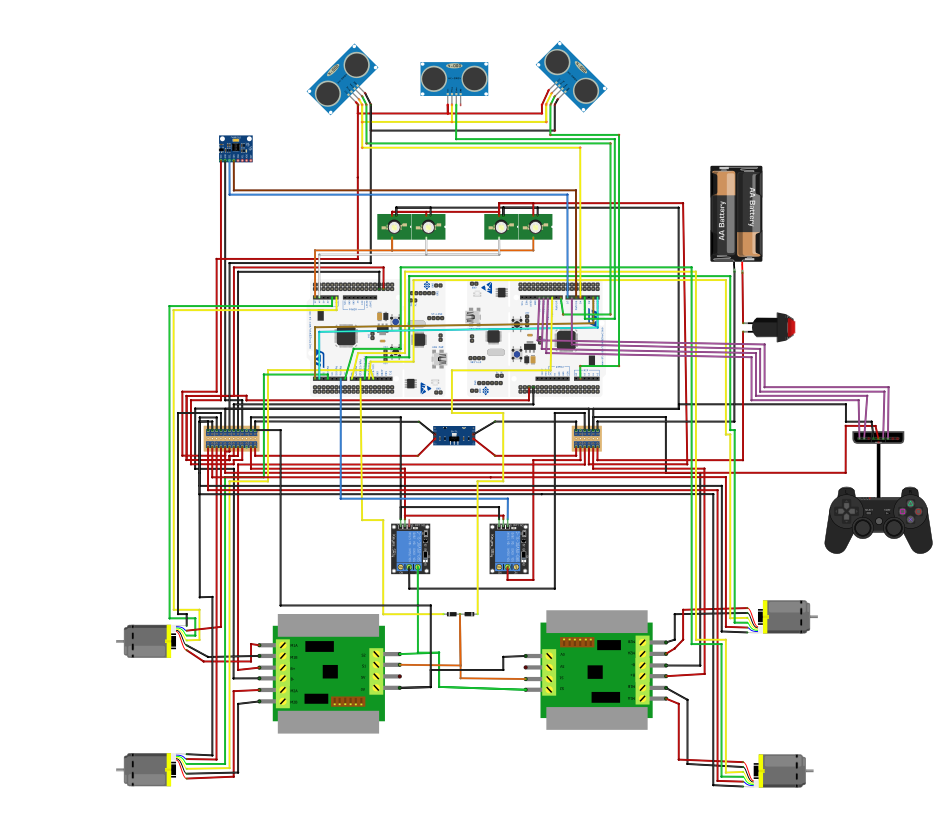
\includegraphics[width=0.85\linewidth]{image/friz.png}
\caption{\label{fig:friz}Panoramica dei componenti del Rover in Fritzing.}
\end{figure}
Il rover è governato da due schede elettroniche che comunicano tra loro per scambiarsi dati. Questa doppia configurazione garantisce una maggiore sicurezza, poiché in caso di guasto di una delle due schede, l'altra può continuare a gestire le operazioni del rover.

Il rover è progettato per rispondere ai comandi impartiti da un operatore tramite un joystick. La marica  può essere impostata in diverse modalità ed è possibile accedere ad un sistema di illuminazione per garantire una navigazione sicura anche in condizioni di scarsa visibilità.

Per quanto riguarda i sistemi di protezione, il rover è dotato di tre sensori ad ultrasuoni posizionati sulla parte anteriore e disposti in modo da coprire un angolo di 45° ciascuno. Questi sensori permettono al rover di rilevare eventuali ostacoli sul percorso e di fermarsi per evitare collisioni.

Inoltre, il rover è equipaggiato con due sensori di temperatura che interrompono il funzionamento del sistema nel caso in cui la temperatura superi una certa soglia critica. Questo è fondamentale per prevenire danni ai componenti elettronici causati da un eccessivo riscaldamento.

Il rover dispone anche di un sensore di accelerazione e di encoder, che forniscono feedback sul corretto funzionamento dei motori. Infine, è presente un sensore di batteria che avverte l'utente quando il livello di carica è troppo basso, prevenendo così interruzioni impreviste del funzionamento del rover.

\newpage

\section{Alimentazione}
L'alimentazione del rover è fornita da una batteria Gens ace a al litio-polimero . Questa batteria ha un voltaggio di 11.1 V, una capacità di 2200 mAh. La batteria in esame è formta da 3 celle ricaricabbili ripettivamente da 3.7 V l'una.
\begin{figure}[H]
\centering

\includegraphics[width=0.7\linewidth]{image/batteria.png}
\caption{\label{fig:batteria}Batteria Gens.}
\end{figure}
Da notare che un sistema di ricarica non adatto potrebbe creare squilibri di carica fra le celle e portare a consegueze spiacevoli: 
\begin{itemize}
\item Durata della batteria: Se le celle non sono caricate in modo uniforme, alcune celle potrebbero essere sovraccaricate mentre altre potrebbero non essere completamente caricate. Questo può ridurre la durata complessiva della batteria. 
\item  Prestazioni ottimali: Per ottenere le migliori prestazioni da una batteria, tutte le celle devono essere alla stessa tensione. Se una cella è a una tensione inferiore, può limitare la quantità di energia che la batteria può fornire.
\item Sicurezza: Sovraccaricare oC sottocaricare le celle di una batteria può essere pericoloso e può portare a guasti della batteria o, nel peggiore dei casi, a incendi.
\end{itemize}
L'alimentazione a 12V viene utilizzata per fornire energia ai motori , alle relative schede di controllo e al sistema di illuminazione.
L'alimentazione può essere interrotta in qualsiasi momento grazie ad un apposito pulsante posto sul retro del rover.
La maggior parte della sensoristica lavora a 5V dunque si è utilizzato un modulo di step-down che porta l'alimentazione da 12V in ingresso a 5 in uscita.

\begin{figure}[H]
\centering
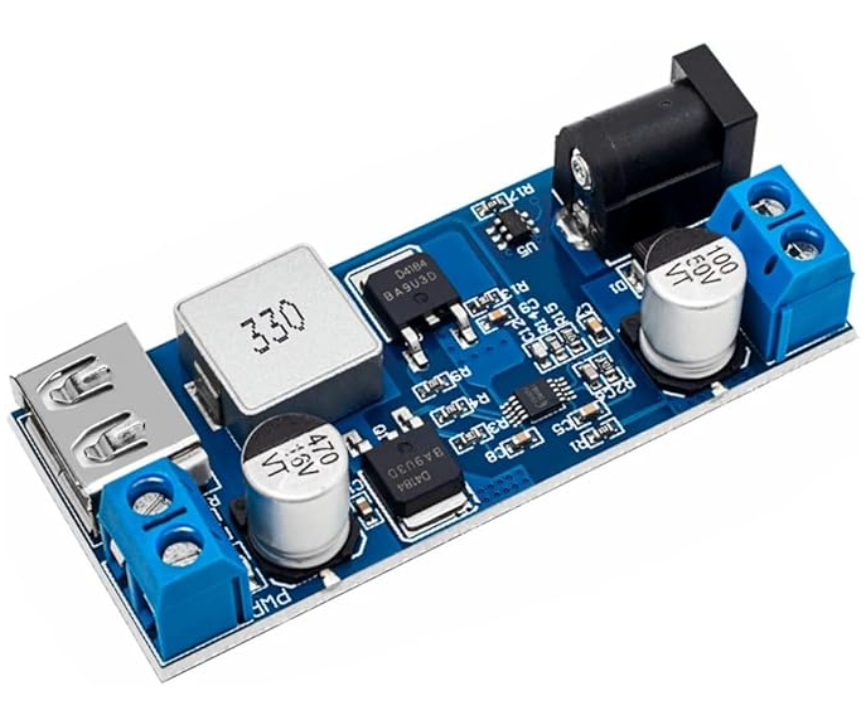
\includegraphics[width=0.6\linewidth]{image/step-down.png}
\caption{\label{fig:step-down}Modulo di step-down.}
\end{figure}
Dal modulo di Step-Down partono dei cavi che vanno verso più morsettiere che smistano la corrente ai vari sensori.
Le schede di controllo STM32 sono alimentate a 5V dal modulo di Step-Down e hanno vari pin per l'alimentazione. Nello specifico si è utilizzato il pin che eroga una tensione di 3,3 V in uscita  per l'alimentazione del ricevitore del controller PS2.
Il cablaggio è stato effettuato scegliendo opportunamente la sezione dei cavi in base alla corrente che andrà a fluirvi e anche in base alle sollecitazioni alle quali il cavo deve resistere.
\newpage

Qui riportato lo schema di cablaggio del Rover:

\begin{figure}[H]
\centering
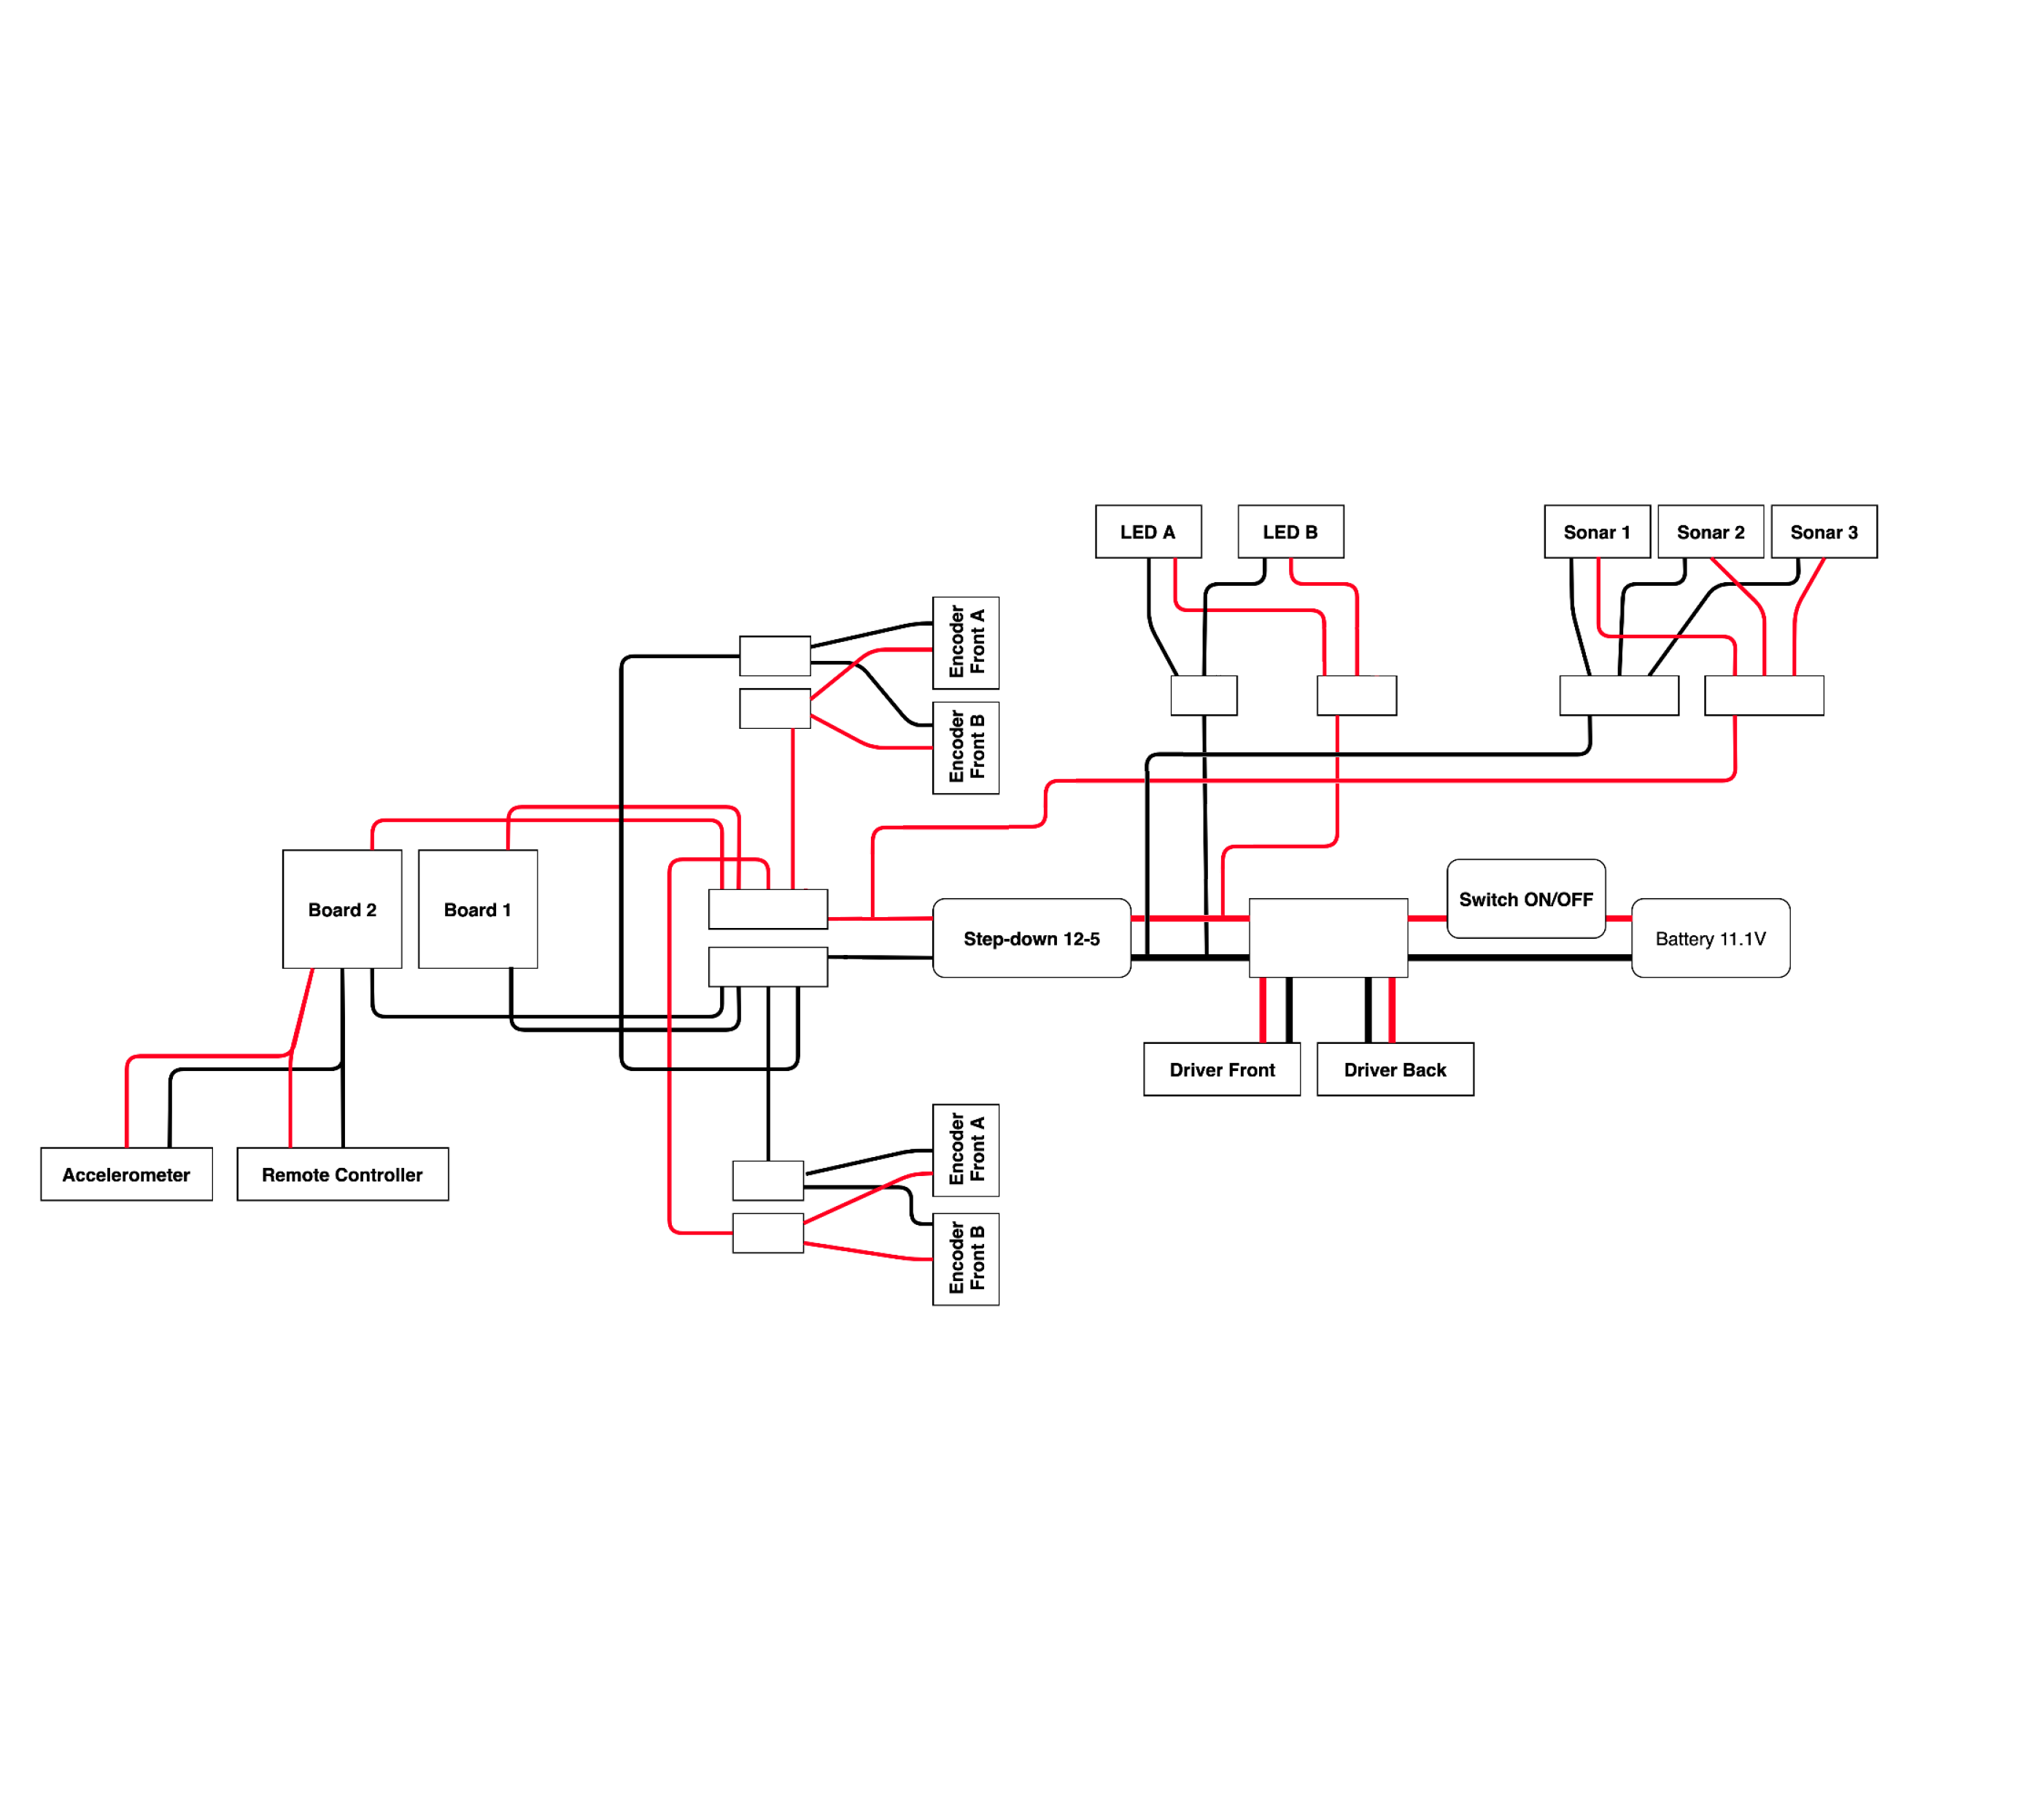
\includegraphics[width=1\linewidth]{image/alimentazione.png}
\caption{\label{fig:alimentazione}Schema di alimentazione.}
\end{figure}
\newpage

\section{STM32}
Per la gestione della sensoristica e della parte di attuazione sono presenti due schede STM32F401RE rispettivamente col ruolo di master e di slave.
Le due schede comunicano tra di loro tramite protocollo i2c scambiandosi messaggi utili per l'attuazione e per la rilevazione di eventuali soglie critiche. La presenza della doppia scheda permette al rover di essere più resiliente alla rottura e/o al malfunzionamento di una scheda infatti sia la master che la slave possono fermare la corsa del rover e ipedire eventuali urti o surriscaldamenti pericolosi.

\begin{figure}[H]
\centering
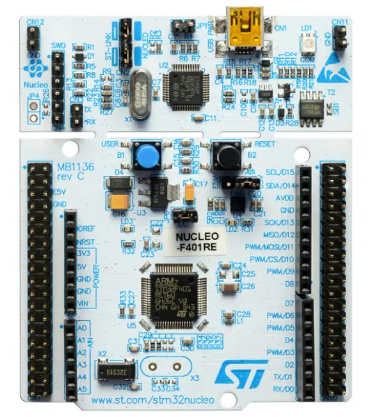
\includegraphics[width=0.5\linewidth]{image/stm32.png}
\caption{\label{fig:STM32}STM32f401re.}
\end{figure}

La STM32F401RE è un microcontrollore ad alte prestazioni basato sul core ARM® Cortex®-M4 32-bit RISC che opera ad una frequenza fino a 84 MHz. Qui riportate alcune specifiche tecniche:
\begin{itemize}
\item Core: ARM® 32-bit Cortex®-M4 CPU con FPU, acceleratore in tempo reale adattivo (ART Accelerator™) che consente l'esecuzione da memoria Flash senza attesa, frequenza fino a 84 MHz.
\item Memorie: fino a 512 Kbytes di memoria Flash e fino a 96 Kbytes di SRAM.
\item Consumo energetico: Run: $146 \mu A/MHz$ (periferico spento), Stop (Flash in modalità Stop, tempo di risveglio rapido): $42 \mu A$.

\item Convertitore A/D: 1×12-bit, 2.4 MSPS fino a 16 canali.
\item Timer: fino a 11 timer: fino a sei 16-bit, due timer 32-bit fino a 84 MHz.
\item Debug: debug seriale (SWD) , interfacce JTAG.
\item I/O: fino a 81 porte I/O con capacità di interruzione.
\end{itemize}
\newpage

\section{Sensori}
\subsection{Ultrasuoni}
Per determinare la presenza di ostacoli nel senso di marcia il rover monta 3 sensori ad ultrasound disposti con 45° di sfasamento l'uno dall'altro . Questa configurazione permette di individuare anche gli ostacoli al lati e consente ,in caso di pericolo, di svoltare verso un eventuale lato libero.
\begin{figure}[H]
\centering
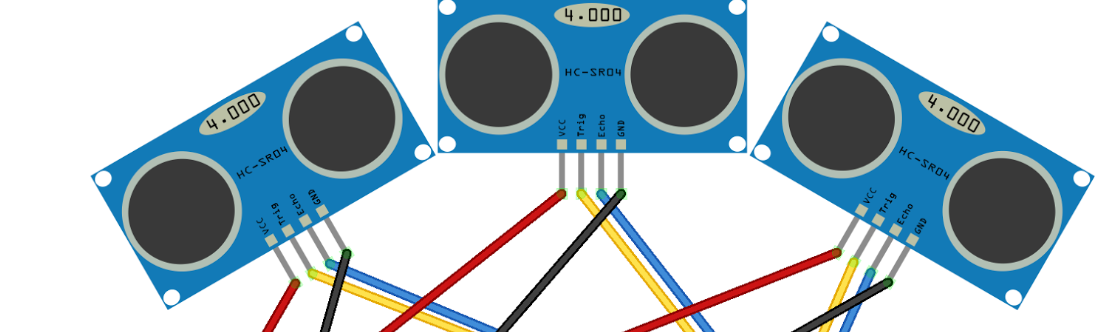
\includegraphics[width=0.6\linewidth]{image/ultra.png}
\caption{\label{fig:ultra}Disposizione Ultrasound.}
\end{figure}
Il modulo HC-SR04 è un sensore di distanza ad ultrasuoni molto utilizzato nell'elettronica. Ecco come funziona:
\begin{enumerate}
\item  Il trasmettitore ad ultrasuoni (pin Trig) emette un suono ad alta frequenza (40 kHz).
\item Il suono viaggia attraverso l'aria.
\item Se trova un oggetto, rimbalza indietro verso il modulo.
\item Il ricevitore ad ultrasuoni (pin Echo) riceve il suono riflesso (echo).
\item Tenendo conto della velocità del suono nell'aria e del tempo di viaggio (il tempo trascorso tra la trasmissione e la ricezione del segnale) possiamo calcolare la distanza da un oggetto utilizzando la seguente formula:$$\text{Distanza} = 0.03431 \times t / 2$$
Dove $t$ è il tempo che intercorre tra l'emissione del segnale sonoro ed il suo ritorno. Questa formula deriva dal fatto che la velocità del suono nell'aria a \(20^\circ C\) è di \(343.1 m/s\), che convertita diventa \(0.03431 cm/\mu s\). Il tempo viene diviso per \(2\) perché la distanza percorsa dal suono è doppia rispetto alla distanza dell’ostacolo, in quanto l’impulso sonoro deve andare verso l’ostacolo e tornare indietro.

\end{enumerate}
\begin{figure}[H]
\centering
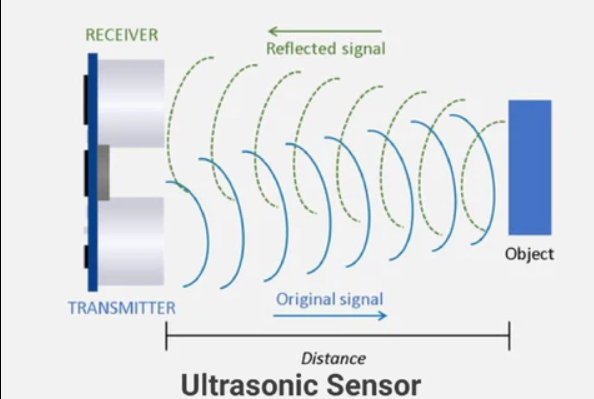
\includegraphics[width=0.6\linewidth]{image/ultrafunc.png}
\caption{\label{fig:ultrafunc}Funzionamento Ultrasound.}
\end{figure}

Qui riportate alcune caratteristiche tecniche:
\begin{itemize}
    \item Tensione di lavoro: 3 - 5.5 Vdc.
    \item Corrente assorbita: circa 3 mA.
    \item Frequenza di lavoro: 40 kHz.
    \item Distanza minima: 2 cm.
    \item Distanza massima: 400 cm.
    \item Risoluzione: 3 mm.
    \item Angolo di misura: 15 - 20°.
\end{itemize}

\begin{figure}[H]
\centering
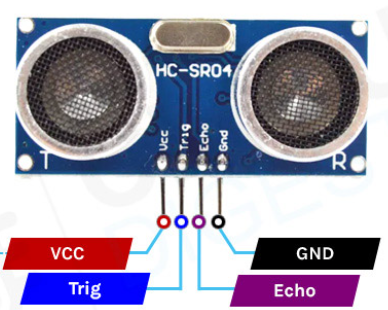
\includegraphics[width=0.6\linewidth]{image/pinoutultra.png}
\caption{\label{fig:pinoutultra}Pinout Ultrasound.}
\end{figure}
Il modulo HC-SR04 dispone di 4 pin:

\begin{itemize}
    \item Vcc: viene collegato alla tensione di alimentazione da 3 a 5.5 V.
    \item Trig: è il pin "Trigger" che deve essere portato alto per inviare il segnale ad ultrasuoni.
    \item Echo: è il pin che produce un impulso che si interrompe quando viene ricevuto il segnale riflesso dall’ostacolo.
    \item GND: viene collegato al GND.
\end{itemize}

\subsection{MPU6050}
\begin{figure}[H]
\centering
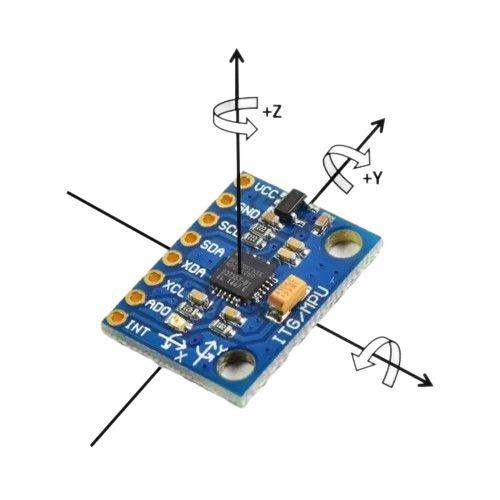
\includegraphics[width=0.6\linewidth]{image/giroscopio.png}
\caption{\label{fig:giroscopio}Giroscopio.}
\end{figure}
Il modulo MPU6050 è un'unità di misura inerziale (IMU) con 6 gradi di libertà (DoF). Questo modulo integra un accelerometro a 3 assi e un giroscopio a 3 assi.
\vspace{0.1cm}

\textbf{Accelerometro}: Misura l'accelerazione, cioè la variazione di velocità per unità di tempo. Gli accelerometri usano parametri di forza e massa dell'oggetto per funzionare. Utilizzano le tecniche MEMS (Micro Electro Mechanical Systems) per misurare le accelerazioni.

I sensori di accelerazione MEMS sono realizzati su un substrato di silicio o di altro materiale semi-
conduttore. La struttura principale del sensore `e una piccola massa sospesa all’interno del dispositivo,
chiamata ”massa di prova” o ”massa sismica.” Questa massa `e sospesa da molle microscopiche e pu`o
muoversi in risposta all’accelerazione. Quando la massa si muove in risposta di uno spostamente si ha
che i condensatori avranno capacit`a diverse da quelle iniziali tramite un circuito si determina qunato
velocemente il condensatore ha cambiato capacit`a.

\begin{figure}[H]
\centering
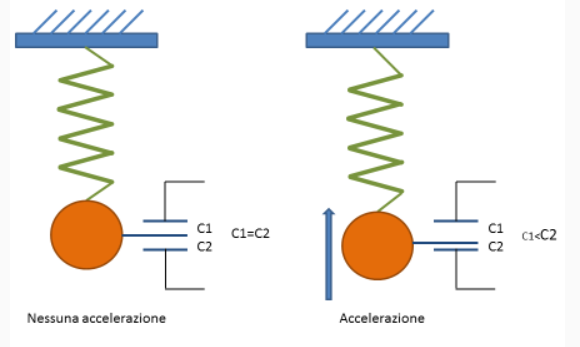
\includegraphics[width=0.82\linewidth]{image/acc.png}
\caption{\label{acc:pot} Esempio di sensore di accelerazione.}
\end{figure}

Chiaramente in base al sistema che abbiamo le dimensioni dei condensatori cambiano in un tipico
accelerometro MEMS le masse mobili sono dell’ordine del milionesimo di grammo, gli spostamenti
delle molle pari alle dimensioni di qualche decina o centinaia di atomi e le fluttuazioni di carica nei
condensatori dell’ordine di una decina di elettroni.\\

\textbf{Giroscopio}: Misura la velocità angolare di un oggetto, ovvero lo spostamento angolare per unità di tempo o la velocità con cui un corpo ruota attorno al proprio asse. Anche in questo caso, le tecniche MEMS vengono utilizzate per misurare la velocità angolare.

 I sensori giroscopici MEMS sfruttano il principio della conservazione del momento angolare. In altre parole, un corpo in rotazione tende a mantenere la sua velocità angolare e la sua direzione di rotazione, a meno che una forza esterna non agisca su di esso.Un giroscopio MEMS è costituito da una piccola massa sospesa all'interno del dispositivo, simile a un pendolo. Questa massa è libera di ruotare attorno a un asse, ed è collegata a un set di microscopiche strutture meccaniche .Quando il dispositivo subisce una rotazione, la massa all'interno del giroscopio tende a mantenere la sua direzione originale a causa della conservazione del momento angolare. Questo movimento della massa è rilevato dal sensore giroscopico, che converte la velocità angolare in un segnale elettrico.Si misura il cambiamento nella capacità tra due superfici quando la massa all'interno del giroscopio si sposta.
 \begin{figure}[H]
\centering
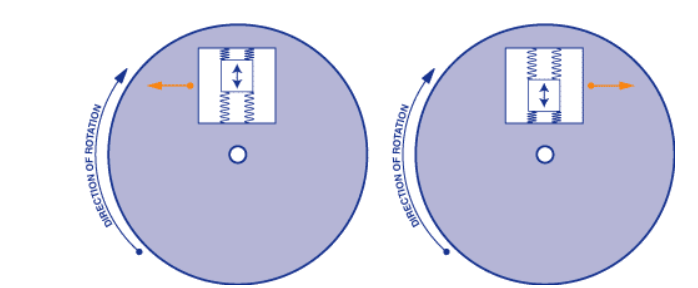
\includegraphics[width=0.82\linewidth]{image/giro.png}
\caption{\label{gito:pot} Esempio di Giroscopio.}
\end{figure}

Il modulo MPU6050 fornisce misurazioni precise in quanto ha un convertitore digitale a 16 bit per ciascun canale e cattura allo stesso tempo x, y e z. Il sensore usa un bus I2C per comunicare .

Questo modulo può essere utilizzato per rilevare il movimento o la posizione di un oggetto, ad esempio, in applicazioni di navigazione, goniometria, stabilizzazione, controllo dei gesti.
Nell'ambito del rover questo sensore è essenziale per effettuare una frenata di emergenza che viri automaticamente verso un lato e  garantisce che i motori funzionino in quanto è possibile rilevare l'accelerazione del veicolo.
Ecco alcune specifiche del modulo MPU6050:

\begin{itemize}
    \item Chip con Convertitore AD a 16 bit Integrato: Questo modulo è molto preciso, in quanto ha un convertitore ADC (da analogico a digitale) da 16 bit per ogni canale.
    \item Range di misura giroscopio: Il giroscopio ha un range di misura di ±250, 500, 1000 e 2000°/s.
    \item Range di misura accelerometro: L’accelerometro ha un range di misura di +2, +4 , +8 , +16 g.
    \item Interfaccia: Il modulo MPU6050 utilizza il protocollo di comunicazione standard I²C.
    \item Alimentazione: Il modulo può essere alimentato con una tensione da 3V a 5V.
\end{itemize}
\subsection{Encoder}
Gli encoder rotativi sono dispositivi elettromeccanici progettati per controllare la posizione e la velocità angolare del movimento
degli assi meccanici.
Esistono diverse varianti di encoder, tra cui quelli che utilizzano sensori magnetici o ottici.
Gli encoder magnetici utilizzano un sistema di rilevazione dei segnali basato sulla variazione del flusso magnetico generato da
un magnete (una o più coppie polari) posto in rotazione di fronte al sensore generalmente fissato all’albero dell’encoder. La
variazione del campo magnetico viene campionata dal sensore e trasformata in un impulso elettrico che definisce la posizione.
Il vantaggio del sistema magnetico è principalmente l’assenza di contatto nella rilevazione, fattore che previene l’usura del
dispositivo e risulta quindi vantaggioso dal punto economico, in quanto non richiede manutenzione ed ha una durabilità
potenzialmente infinita.
Gli encoder magnetici sono particolarmente adatti all’applicazione in ambienti gravosi che richiedono
un’elevata robustezza, velocità e resistenza termica, garantendo al tempo stesso un’affidabilità ottimale nella generazione dei
segnali.
\begin{figure}[H]
\centering
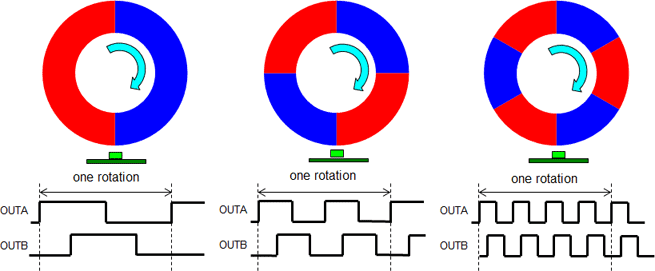
\includegraphics[width=0.82\linewidth]{image/encoder.png}
\caption{\label{encoder:pot} Esempio di funzionamento encoder.}
\end{figure}

La risoluzione di un encoder può essere misurata in vari modi, come ad esempio PPR (Pulse Per Revolution), CPR (Count Per
Revolution).
PPR (Pulse Per Revolution): Questo termine descrive il numero di impulsi (considerando solo la porzione alta dell’onda
quadra) che gli encoder generano su una delle due uscite a onda quadra.
CPR (Count Per Revolution): Questo termine descrive il comportamento dell’encoder ,in particolare i canali A e B generano
un’uscita a 2 bit che ha quattro possibili stati, quindi il CPR (nell’accezione di Count Per Revolution) è pari a quattro volte PPR.
Quindi, la differenza principale tra CPR e PPR negli encoder riguarda il modo in cui vengono conteggiati gli impulsi o i cicli per ogni
rivoluzione.
Nel caso in esame si ha un encoder che produce 48 CPR dunque 12 PPR.
Un encoder rotativo di tipo incrementale è dotato in uscita di due canali, A e B. Questi canali producono uscite a onda quadra e, in
un encoder in quadratura, le due uscite sono sfasate di 90°.
Canale A e Canale B: La relazione di fase tra i canali A e B indica la direzione della rotazione. Con la lettura di un solo canale
si ottiene l’informazione relativa alla velocità di rotazione, mentre mediante l’acquisizione ulteriore del segnale B può essere
discriminato il senso di rotazione in base alla sequenza degli stati prodotti dai due segnali. Per l’encoder preso in esame se il
canale A precede il canale B si ha un senso di rotazione antiorario viceversa se il B precede il canale A.
In pratica, i canali di un encoder sono utilizzati per misurare la direzione di rotazione, la velocità e lo spostamento angolare.
\begin{figure}[H]
\centering
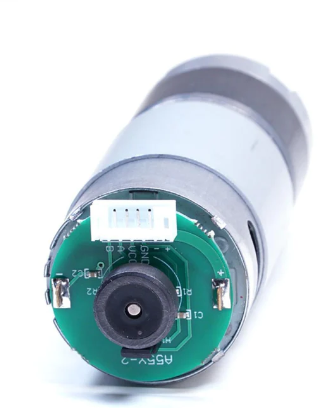
\includegraphics[width=0.7\linewidth]{image/encodermotore.png}
\caption{\label{encodermotore:pot}Encoder montato sul Rover.}
\end{figure}
Nel contesto del rover gli encoder vengono utilizzati per avere un feedback circa la velocità dei motori e poterli pilotare in modo più agevole.Gli encoder danno anche un livello di sicurezza in più in quanto se i motori non dovessero più accettare comandi si potrebbe rilevare questo malfunzionamento leggendo il valore di output degli encoder.
\subsection{PS2 (PlayStation 2) Controller}
Il controller wireless PS2 è un controller standard per la PlayStation 2 ed è identico al controller DualShock originale per la console PlayStation. Dispone di dodici pulsanti analogici (sensibili alla pressione) , cinque pulsanti digitali  e due stick analogici. Il controller dispone anche di due motori di vibrazione, quello sinistro è più grande e potente di quello destro. È alimentato da due batterie AAA. Comunica con la console utilizzando il protocollo RF a 2,4 GHz.
\begin{figure}[H]
\centering
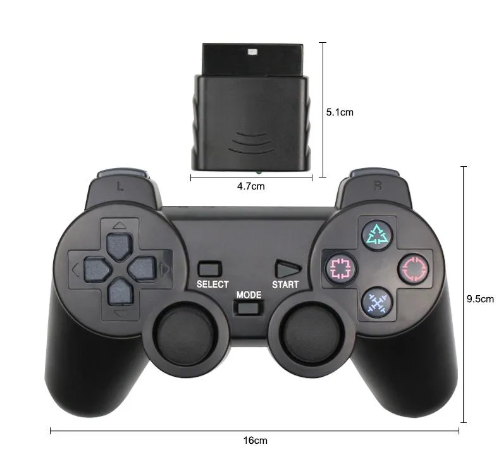
\includegraphics[width=0.7\linewidth]{image/joystick.png}
\caption{\label{joystick:pot} Joystick PS2.}
\end{figure}


Il controller wireless PS2 comunica con i microcontrollori SPI. La PlayStation invia un byte contemporaneamente mentre ne riceve uno (full duplex) tramite comunicazione seriale. C'è un clock (SCK) per sincronizzare i bit di dati attraverso due canali: DATA e CMD. Inoltre, c'è un canale "Attention" (ATT) che dice allo slave se è "attivo" e dovrebbe ascoltare i bit di dati che passano attraverso il canale CMD, o inviare bit di dati attraverso il canale DATA (Ragionevolmente, solo un dispositivo slave dovrebbe essere attivo alla volta). La PlayStation 2 in realtà utilizza questo più una linea aggiuntiva che non fa parte specificamente del protocollo SPI - una linea di "Acknowledge" (ACK).

Il clock è mantenuto alto fino a quando deve essere inviato un byte. Quindi scende basso (attivo basso) per avviare 8 cicli durante i quali i dati vengono inviati e ricevuti simultaneamente. Dopo che ogni comando è ricevuto dal controller, quel controller deve abbassare ACK per almeno un ciclo di clock. Se un controller selezionato non risponde con un ACK, la PS2 ipotizzerà che non ci sia alcun controller presente. I LSB (bit meno significativi) vengono trasmessi per primi.

\begin{figure}[H]
\centering
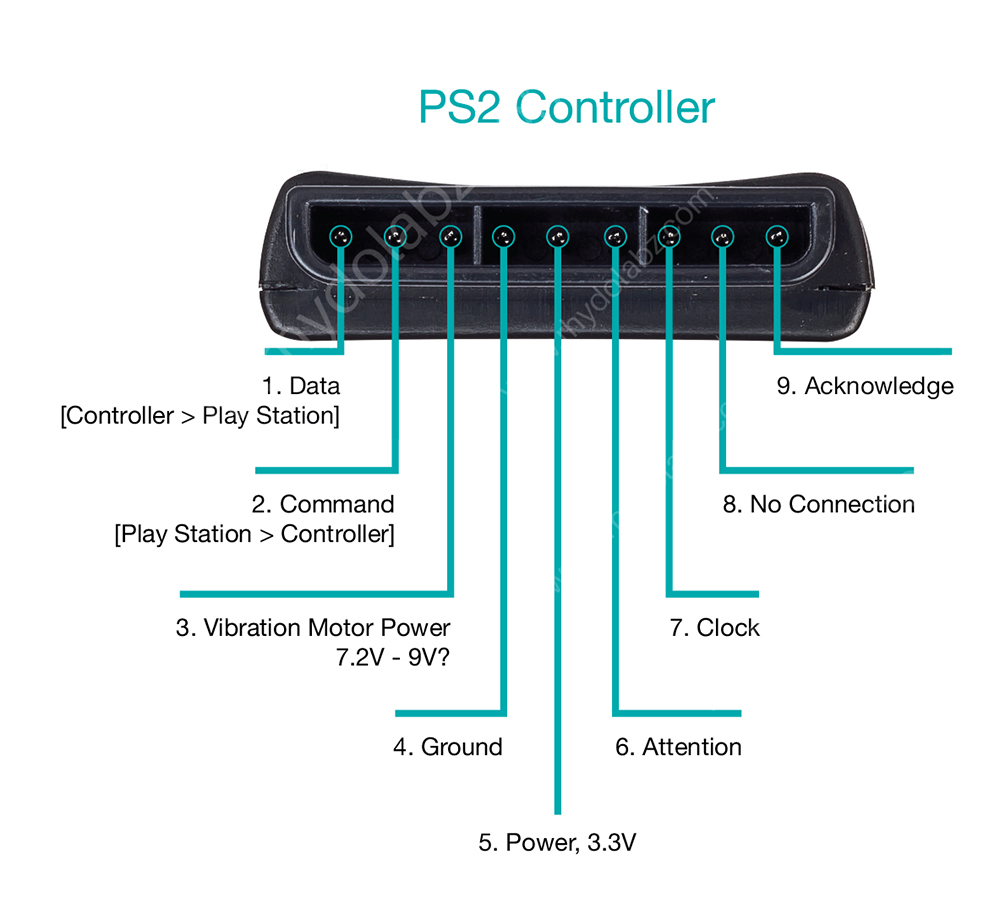
\includegraphics[width=0.7\linewidth]{image/ps2.jpg}
\caption{\label{ps2:pot}Pinout del Ricevitore.}
\end{figure}
Ci sono 9 fili, di cui 6 sono necessari al minimo per comunicare con il controller: (clock, dati, comando, alimentazione e terra, attenzione). Per far funzionare i motori di vibrazione, è anche necessario il filo motor\_power.

\begin{itemize}
    \item \textbf{Dati} : Controller -> PlayStation. Questo è un output a collettore aperto e richiede una resistenza di pull-up (da 1 a 10k). (È necessaria una resistenza di pull-up perché il controller può solo collegare questa linea a terra; non può effettivamente mettere tensione sulla linea).
    \item \textbf{Comando}: PlayStation -> Controller.
    \item \textbf{Alimentazione motori di vibrazione} : 6-9V.
    \item \textbf{GND} :Terra.
    \item \textbf{Alimentazione} : 3.3v.
    \item \textbf{Attenzione} : Questa linea deve essere portata bassa prima di inviare/ricevere ogni gruppo di byte e quindi riportata alta dopo.
    \item \textbf{Clock}: 500kHz, normalmente alto. La comunicazione lavora fra i 100kHz fino a 500kHz .
    \item \textbf{unknown} .
    \item \textbf{ACK} : Questa linea normalmente alta scende bassa circa 12µs dopo ogni byte per mezzo ciclo di clock, ma non dopo l'ultimo bit in un set. Questo è un output a collettore aperto e richiede una resistenza di pull-up (da 1 a 10k).
\end{itemize}
La comunicazione fra controller e joystick avviene tramite pacchetti:

I pacchetti iniziano sempre con un'intestazione di 3 byte. Il primo byte di trasmissione è l'indirizzo per selezionare il controller (0x01) o la memory card (0x81). Il secondo byte di trasmissione è il comando inviato dalla console. Il secondo byte di ricezione ha il nibble superiore che rappresenta l'ID del periferico. Il nibble inferiore è la dimensione dell'output in DWORD (uint16\_t). Il terzo byte di ricezione è sempre 0x5A e segnala la fine dell'intestazione. L'intestazione è seguita dal payload che corrisponde sempre alla dimensione riportata nel secondo byte di ricezione, anche quando non tutti i dati sono utilizzati. I byte di trasmissione non utilizzati sono impostati su 0x00 dalla PSX e su 0x5A dalla PS2.
Esempio per la lettura di pulsanti premuti sul joystick:
\begin{figure}[H]
\centering
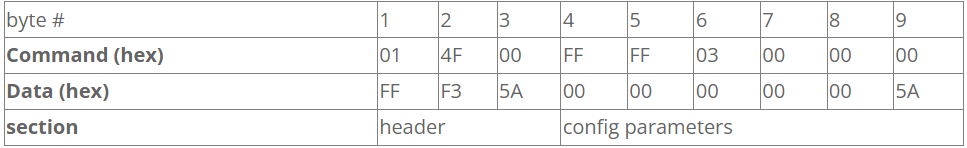
\includegraphics[width=0.9\linewidth]{image/example.png}
\caption{\label{example:pot}Example of command.}
\end{figure}
\subsection{Sensore di batteria}
Per controllare il livello della batteria si è deciso di utilizzare la ADC della STM32.
Qui riportati i passi per la lettura della percentuale di batteria:

\begin{itemize}
    \item Utilizzo di una resistenza per abbassare la tensione: Poiché la tensione fornita dalla batteria è di 12,6 V e l'ADC dello STM32 può gestire una tensione massima di 3,3 V, è necessario ridurre la tensione di ingresso. Questo viene fatto utilizzando una resistenza in serie, formando un partitore di tensione. La tensione in uscita dal partitore di tensione dipende dalla resistenza della batteria e dalla resistenza utilizzata nel partitore di tensione.
    Per portare la tensione della batteria da 12,6 V a 3,3 V, possiamo scegliere i seguenti valori per le resistenze:
\[ R1 = 10 \, k\Omega \]
\[ R2 = 3,3 \, k\Omega \]

Possiamo calcolare la tensione di uscita utilizzando la formula del partitore di tensione:
\[ V_{out} = 12,6 \times \frac{3,3}{10 + 3,3} = 12,6 \times \frac{3,3}{13,3} = 3,15 \, \text{V} \]

Questo valore è abbastanza vicino a 3,3 V.

    \item Mappatura dei valori dell'ADC in percentuale di batteria: Una volta che la tensione di ingresso è stata adattata alla gamma di tensioni dell'ADC, è possibile leggere la tensione utilizzando l'ADC dello STM32. I valori letti dall'ADC rappresentano la tensione in ingresso, che a sua volta riflette lo stato di carica della batteria. Si è mappata la tensione letta dall'ADC in percentuale di carica della batteria utilizzando una relazione lineare . 

\end{itemize}


\subsection{Temperatura}
Il sensore di temperatura interno della STM32 è un dispositivo che permette di misurare la temperatura interna del microcontrollore. Questo sensore è molto utile per monitorare le condizioni di funzionamento del chip e prevenire eventuali problemi dovuti al surriscaldamento.
Qui riportato il funzionamento del sensore e l'interfacciamento con la stm32:

\begin{enumerate}
    \item Abilitazione del sensore: Prima di tutto, è necessario abilitare il sensore di temperatura interno. Questo si fa tramite la configurazione dei registri ADC (Analog to Digital Converter) della STM32.
    \item Lettura del valore: Una volta abilitato il sensore, si può iniziare a leggere i valori di temperatura. Questo si fa avviando una conversione ADC e leggendo il valore risultante.
    \item Conversione del valore: Il valore letto dall’ADC non è direttamente la temperatura in gradi Celsius. Per ottenere la temperatura, è necessario convertire il valore ADC utilizzando le costanti fornite dal produttore.
\end{enumerate}
\newpage

\section{Attuatori}
\subsection{Driver Motori }
Un driver per motori DC è un dispositivo che regola la velocità e la direzione di un motore a corrente continua controllando la quantità di corrente fornita al motore. Può essere integrato direttamente in alcuni dispositivi elettronici o può essere un componente separato che si connette al motore e ad altri circuiti di controllo.

I driver per motori DC hanno diversi componenti e funzioni chiave:
\begin{enumerate}
    \item Controllo della velocità e direzione: Il driver regola la velocità del motore variando la quantità di corrente che fluisce attraverso di esso. Per invertire la direzione del motore, il driver può invertire il flusso di corrente.
    \item Modulazione della larghezza di impulso (PWM): Molte unità di controllo utilizzano la tecnica PWM per variare la quantità di corrente inviata al motore. La PWM regola la larghezza degli impulsi di corrente inviati al motore, modificando così la sua velocità.
    \item Protezioni e sicurezza: I driver spesso includono meccanismi di protezione come il controllo della temperatura e la limitazione della corrente per evitare danni al motore e al driver stesso. Queste funzionalità aiutano a prevenire surriscaldamenti e danni in situazioni di sovraccarico.
    \item Interfaccia di controllo: Molti driver sono progettati per essere controllati da microcontroller o dispositivi elettronici tramite segnali analogici (tensioni variabili), segnali digitali o protocolli di comunicazione come la seriale.
    \item Regolazione della tensione: Alcuni driver possono avere circuiti integrati per regolare la tensione di alimentazione fornita al motore, garantendo che il motore funzioni a una tensione appropriata.
\end{enumerate}

In sostanza, il driver per motori DC agisce come un intermediario tra il sistema di controllo (spesso un microcontrollore o un processore) e il motore stesso, consentendo un controllo preciso della velocità, della direzione e della potenza del motore DC in diverse applicazioni.

\vspace{0.5cm}

Nello specifico del Rover si è utilizzato il driver Sabertooth 2X12 Motor Controller 2X12A. 
 Questo dispositivo è in grado di alimentare due motori dc
brushed con corrente di 12 Ampere, riuscendo anche a sopportare correnti di 25 ampere per alcuni secondi. Ha un sistema di
protezione da sovracorrente e surriscaldamento che previene seri danni alla scheda e al sistema in generale.
La Sabertooth consente di controllare due motori con tensione analogica, controllo radio, seriale e seriale pacchettizzata. La
modalità di pilotaggio viene selezionata da appositi interruttori DIP presenti sulla scheda .
Il formato del pacchetto per il Sabertooth è composto da un byte di indirizzo, un byte di comando, un byte di dati e un checksum di
sette bit. I byte di indirizzo hanno un valore maggiore di 128, e tutti i byte successivi hanno valori di 127 o inferiori. Questo consente
a diversi tipi di dispositivi di condividere la stessa linea seriale.
In modalità seriale pacchettizzata, l'ingresso S2 è configurato come un arresto di emergenza attivo basso (active-low emergency
stop). Se si desidera un arresto di emergenza, tutti gli ingressi S2 possono essere collegati in serie e portando l'ingresso S2 a
basso si causerà lo spegnimento del driver.
I transistor del Sabertooth vengono commutati a velocità (32kHz) per un funzionamento silenzioso.
La Sabertooth 2x12 dispone di tre LED indicatori.
Il LED verde contrassegnato come Status1 viene utilizzato per comunicare varie informazioni sullo stato attuale. Nella maggior
parte dei casi, Status1 funge da indicatore di alimentazione. In modalità R/C, si illumina debolmente se non è presente alcun
collegamento R/C e intensamente se è presente un collegamento R/C.
Il LED verde contrassegnato come Status2 viene utilizzato in modalità litio. Lampeggia per indicare il numero di celle al litio rilevate.
Inoltre, quando Status2 ed Error lampeggiano contemporaneamente, e non si ha alcuna uscita dai motori, l'unità sta visualizzando
la modalità di bassa tensione.
Il LED rosso Error si illumina se il Sabertooth ha rilevato un problema. Si accenderà se il driver si è spento a causa del
surriscaldamento o della sovracorrente.
\begin{figure}[H]
\centering
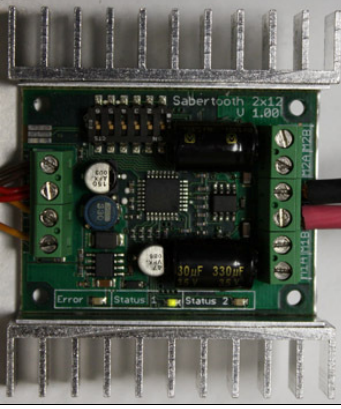
\includegraphics[width=0.7\linewidth]{image/saber.png}
\caption{\label{saber:pot}Sabertooth.}
\end{figure}


Sul lato destro, è evidente l'alimentazione (12 V), mentre ai lati sono presenti le uscite destinate a controllare i motori.
Sul lato sinistro, ci sono quattro morsettiere, dall'alto verso il basso: terra, 5V che può essere utilizzato come input per altri
dispositivi, S1 (canale per la ricezione dei comandi) e S2 (canale per l'arresto di emergenza).
Qui di seguito vengono riportati le caratteristiche salienti del driver:
\begin{itemize}
    \item \textbf{Input voltage}: 6-24V nominale, 30V massima.
    \item\textbf{Output current}: Fino a 12 A per canale. Carichi di picco possono raggiungere fino a 25A per canale per alcuni secondi.
\end{itemize}

\subsection{Motori}
Il motore a corrente continua (CC) Brushed è un dispositivo elettrico che trasforma l'energia elettrica in energia meccanica attraverso l'assorbimento di corrente continua e la generazione di rotazione.

Composto da quattro elementi principali - lo statore, il rotore, il commutatore e le spazzole - il motore a CC Brushed presenta un design essenziale. Lo statore, contenente magneti permanenti o elettromagneti, rimane immobile, mentre il rotore, elemento mobile del motore, riceve l'alimentazione esterna mediante corrente continua. I fili di rame avvolti sono collegati al commutatore, un interruttore rotante, che fornisce loro l'energia necessaria.

L'accensione e lo spegnimento sequenziali delle bobine generano un campo magnetico rotante. Questo campo interagisce con i diversi campi dei magneti fissi nello statore, creando la coppia che avvia la rotazione. Tale processo sfrutta le forze di attrazione e repulsione dei poli magnetici per convertire l'energia elettrica della corrente continua in energia meccanica, manifestata attraverso il movimento rotatorio.
\begin{figure}[H]
\centering
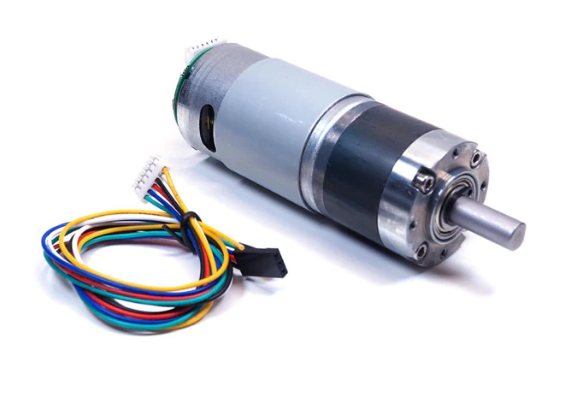
\includegraphics[width=0.7\linewidth]{image/motore.png}
\caption{\label{motore:pot}Motore.}
\end{figure}
Il motore utilizzato per il rover è il \textbf{LynxMotion 36GP-540-51-EN} e presenta le seguenti caratteristiche:

\begin{itemize}
    \item \textbf{Tensione nominale:} 12 V
    \item \textbf{Corrente:}
    \begin{itemize}
        \item Senza carico: 0.5 A
        \item Stallo: 3 A
    \end{itemize}
    \item \textbf{Velocità:}
    \begin{itemize}
        \item Senza carico: 170 rpm ± 10\%
        \item A coppia nominale: 145 rpm ± 10\%
    \end{itemize}
    \item \textbf{Coppia:}
    \begin{itemize}
        \item Nominale: 11.5 kg cm
        \item Stallo: 78 kg cm
    \end{itemize}
    \item \textbf{Encoder:}
    \begin{itemize}
        \item Tensione: 5 V
        \item PPR (Pulse per Revolution): 12
        \item Frequenza massima: 800 kHz
        \item Tipo di segnale: Onda quadra AB a 90°
    \end{itemize}
\end{itemize}


La sequenza di cablaggio per il motore e l’encoder è la seguente: il filo giallo è collegato al polo positivo del motore, il filo bianco al polo negativo del motore, il filo nero al GND del sensore Hall, il filo rosso al VCC del sensore Hall, il filo blu all’uscita A del sensore Hall e il filo verde all’uscita B del sensore Hall.

\subsection{LED}
Per l'illuminazione della strada sono stati installati sul rover due LED .
Un LED (Light Emitting Diode, ovvero diodo ad emissione di luce) è un componente elettronico che emette luce quando attraversato da corrente elettrica.
In particolare è stato utilizzato il A4WD3-LED Board.
\begin{figure}[H]
\centering
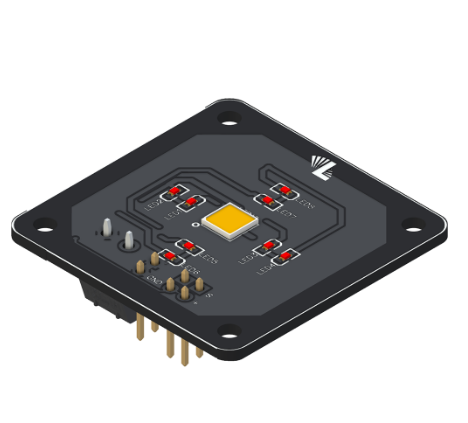
\includegraphics[width=0.55\linewidth]{image/led.png}
\caption{\label{led:pot}LED.}
\end{figure}
 I LED (bianchi o tutti e 8 rossi) possono essere controllati tramite pin di alimentazione o utilizzando i pin digitali a 5V di un microcontrollore. Questo modulo è composto da 1 LED bianco centrale e da 8 rossi , è possibile pilotare indipendentemente i due led e dunque è possibile accendere solo il led bianco mentre i rossi sono spenti.
\newpage

\section{Documentazioni}
\begin{itemize}
    \item \textbf{Batteria}: \href{https://asset.conrad.com/media10/add/160267/c1/-/en/002145181TS00/rapporto-di-prova-2145181-gens-ace-batteria-ricaricabile-lipo-111-v-2200-mah-numero-di-celle-3-45-c-softcase-xt60.pdf}{Battery Datasheet}
    
    \item \textbf{Step-Down}
    \href{https://store.mectronica.it/it/alimentatori/2096-modulo-di-alimentazione-step-down-conversione-di-tensione-da-1224v-a-5-v-5-a.html}{Step-Down Datasheet}
    \item \textbf{STM32f402re}
    \href{https://www.st.com/en/evaluation-tools/nucleo-f401re.html}{STM32f402re Datasheet}
    
    \item \textbf{Ultrasound}
    \href{https://cdn.sparkfun.com/datasheets/Sensors/Proximity/HCSR04.pdf}{Ultrasound Datasheet}
    
    \item \textbf{MPU6050}
    \href{https://invensense.tdk.com/wp-content/uploads/2015/02/MPU-6000-Datasheet1.pdf}{MPU6050 Datasheet}
\item \textbf{Encoder}
    \href{https://cdn.robotshop.com/media/2/2dm/rb-2dm-02/pdf/36gp540-51-en.pdf}{Encoder Datasheet}
    \item \textbf{PS2 (PlayStation 2) Controller}
    \href{https://store.curiousinventor.com/guides/PS2/}{PS2 (PlayStation 2) Controller
 Datasheet}
 \item \textbf{Driver Motori}
\href{https://www.dimensionengineering.com/datasheets/Sabertooth2x12.pdf}{Driver Motori Datasheet}
    \item \textbf{Motore}
    \href{https://cdn.robotshop.com/media/2/2dm/rb-2dm-02/pdf/36gp540-51-en.pdf}{Motore Datasheet}
    \item \textbf{LED}
    \href{https://wiki.lynxmotion.com/info/wiki/lynxmotion/view/servo-erector-set-system/ses-electronics/ses-modules/a4wd3-led-board/#HSpecifications}{LED Datasheet}

\end{itemize}
\part{firmware}
  Il firmware rappresenta il cuore pulsante di ogni rover operante in ambito critico. Questo capitolo si concentra sulla progettazione e implementazione del firmware, un elemento cruciale che governa le funzionalità di base del rover e ne determina le prestazioni e l’affidabilità.

  Il firmware è il software incorporato che controlla le funzioni hardware del rover. Esso fornisce le istruzioni di basso livello per il controllo dei vari componenti e sistemi del rover, tra cui i motori, i sensori, i sistemi di comunicazione e altro ancora.

  In un ambiente critico, la progettazione del firmware deve tener conto di una serie di fattori chiave. Questi includono l’efficienza energetica, la robustezza in condizioni estreme, la capacità di eseguire compiti complessi con precisione e la facilità di aggiornamento e manutenzione.

  In particolare, verranno discusse le scelte di design effettuate per poter raggiungere gli obiettivi di affidabilità e disponibilità del \textit{Rover}, presentando diagrammi ed elaborati \textit{Stateflow} e successivamente analizzando il codice C nel dettaglio, così da avere una chiara ed estensiva comprensione del lavoro svolto.
  \section{Design}
    Per design, si intende il lavoro di progettazione e rifinitura di scelte da implementarsi successivamente e che dovranno riflettere quanto precedentemente ideato. Una progettazione di alto e basso livello ha consentito una efficace parallelizzazione e strutturazione del lavoro, consentendo anche di avere un riscontro costante sulla correttezza di quanto via via implementato. 
    \subsection{Diagrammi UML}
      \subsubsection{Use Case Diagrams: Digital Drive}
        \begin{figure}[h]
          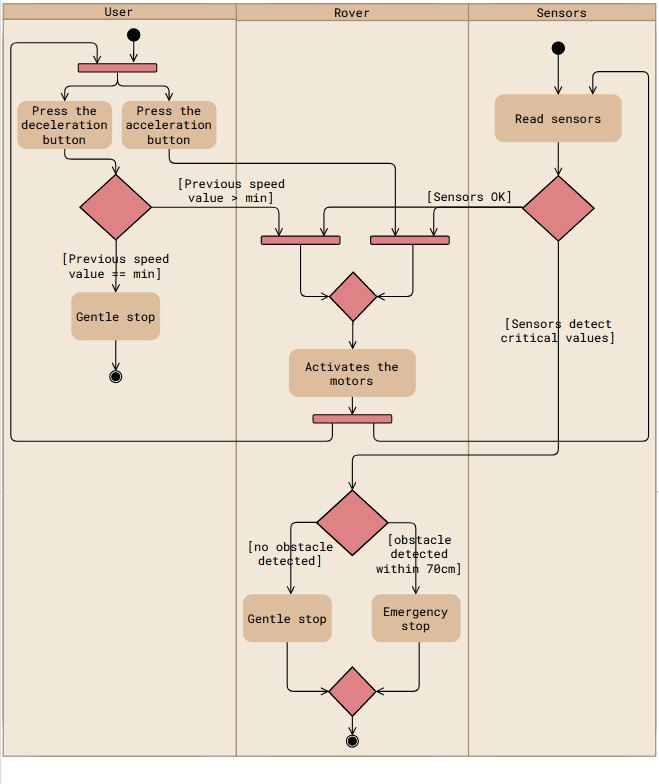
\includegraphics[width=0.7\linewidth]{../Use_Case_Diagram/Digital_Drive.jpg}
          \centering
          \caption{Digital Drive UML}
        \end{figure}
        Il diagramma UML illustra il processo di controllo di un rover utilizzando i pulsanti di un controller, non uno stick analogico. Coinvolge tre entità principali: Utente, Rover e Sensori.

        \begin{itemize}
          \item \textbf{Utente}:
              \begin{itemize}
              \item L'utente ha due opzioni: "Premere il pulsante di decelerazione" o "Premere il pulsante di accelerazione".
              \item Se viene premuto il pulsante di decelerazione e "[Valore di velocità precedente > min]", si arriva a un "Fermata dolce".
              \item Se viene premuto il pulsante di accelerazione e "[Valore di velocità precedente = min]", si procede ad attivare i motori del rover.
              \end{itemize}
          \item \textbf{Rover}:
              \begin{itemize}
              \item Le azioni del rover dipendono sia dall'input dell'utente che dal feedback dei sensori.
              \item Quando i motori sono attivati, ci sono due possibili risultati basati sui dati del sensore: 
                  \begin{enumerate}
                  \item Se "[Sensori OK]", significa che non sono stati rilevati valori critici dai sensori, quindi i motori rimangono attivati.
                  \item Se "[I sensori rilevano valori critici]", viene innescata una fermata di emergenza.
                  \end{enumerate}
              \end{itemize}
          \item \textbf{Sensori}:
              \begin{itemize}
              \item I sensori leggono continuamente i dati.
              \item Svolgono un ruolo cruciale nel determinare se il rover continua il suo movimento o si ferma in caso di emergenza.
              \end{itemize}
          \end{itemize}
          
        Il flusso delle azioni è diretto da frecce che indicano la sequenza delle operazioni in base alle condizioni soddisfatte in ogni punto di decisione (forme di diamante). Ad esempio, premere i pulsanti porta a controlli condizionali come "[Valore di velocità precedente > min]" o letture del sensore come "[Sensori OK]". A seconda che queste condizioni siano vere o false, vengono eseguite diverse azioni come "Fermata dolce", "Attiva i motori" o "Fermata di emergenza".

      \subsubsection{Use Case Diagrams: Analog Drive}
        \begin{figure}[h]
          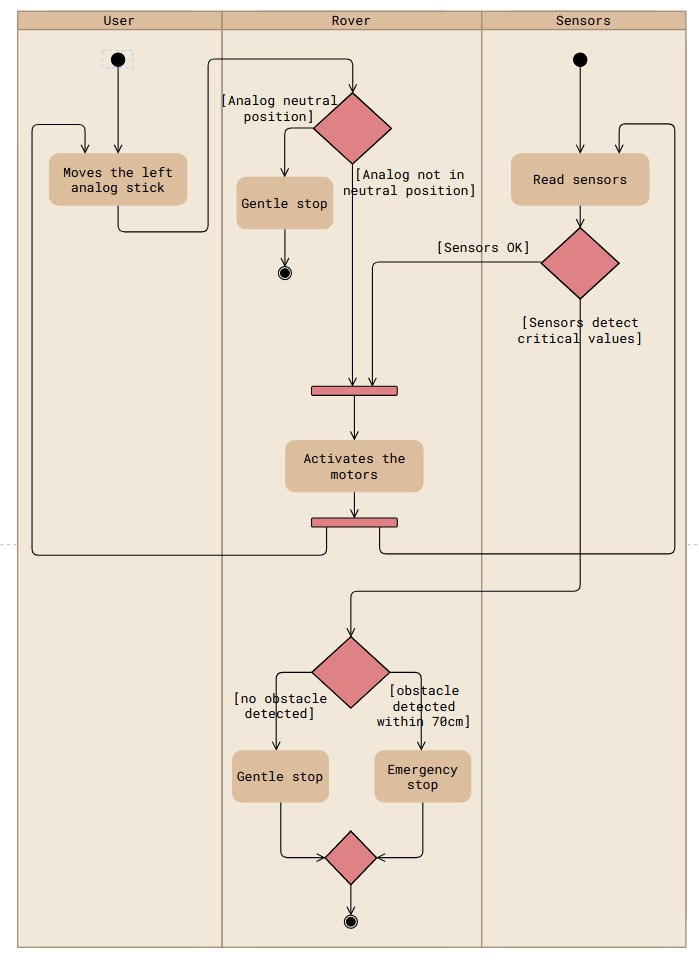
\includegraphics[width=0.7\linewidth]{../Use_Case_Diagram/Drive_Analog.jpg}
          \centering
          \caption{Analog Drive UML}
        \end{figure}

        Si inizia con l’azione dell’utente che muove lo stick analogico sinistro. Questa azione è fondamentale perché attiva i motori del rover, mettendo in moto l’intero sistema.

        A questo punto, il sistema verifica se lo stick analogico è in posizione neutra. Se lo è, il rover esegue una “fermata dolce”, ovvero rallenta gradualmente fino a fermarsi. Questo permette al rover di fermarsi in modo sicuro senza causare danni ai suoi componenti interni.
        
        Se lo stick analogico non è in posizione neutra, il sistema verifica le letture dei sensori. Se i sensori rilevano che tutto è a posto (ovvero, non rilevano valori critici), i motori del rover rimangono attivati e il rover continua a muoversi.
        
        Tuttavia, se i sensori rilevano valori critici, il sistema innesta una “fermata di emergenza”. Questo significa che il rover si ferma immediatamente, indipendentemente dalla sua velocità o direzione attuale. Questa è una misura di sicurezza importante per prevenire danni al rover o al suo ambiente in caso di problemi imprevisti.
        
        Inoltre, il sistema verifica continuamente la presenza di ostacoli entro 7 cm dal rover. Se rileva un ostacolo in questo raggio, innesta una “fermata di emergenza” per evitare una collisione. Se non rileva ostacoli, il rover esegue una “fermata dolce”, rallentando gradualmente fino a fermarsi.
        
        In tutto questo processo, i sensori svolgono un ruolo cruciale. Continuano a leggere i dati e a fornire feedback al sistema, influenzando direttamente le azioni del rover. Se i sensori rilevano un problema, il sistema può reagire di conseguenza per garantire la sicurezza del rover.

        \begin{itemize}
          \item \textbf{Utente}:
              \begin{itemize}
              \item L'utente muove lo stick analogico sinistro.
              \item Questa azione attiva i motori del rover.
              \end{itemize}
          \item \textbf{Rover}:
              \begin{itemize}
              \item Se lo stick analogico è in posizione neutra, c'è una fermata dolce; se non è in posizione neutra e i sensori sono ok, continua l'operazione.
              \item Se i sensori rilevano valori critici, viene innescata una fermata di emergenza.
              \item Se viene rilevato un ostacolo entro 7 cm, si verifica una fermata di emergenza; altrimenti, si verifica una fermata dolce.
              \end{itemize}
          \item \textbf{Sensori}:
              \begin{itemize}
              \item Leggono i valori dei sensori e svolgono un ruolo cruciale nel determinare le azioni del rover in base a tali letture.
              \end{itemize}
        \end{itemize}
          
      \subsubsection{Use Case Diagrams: Obstacle Avoidance}
        \begin{figure}[h]
          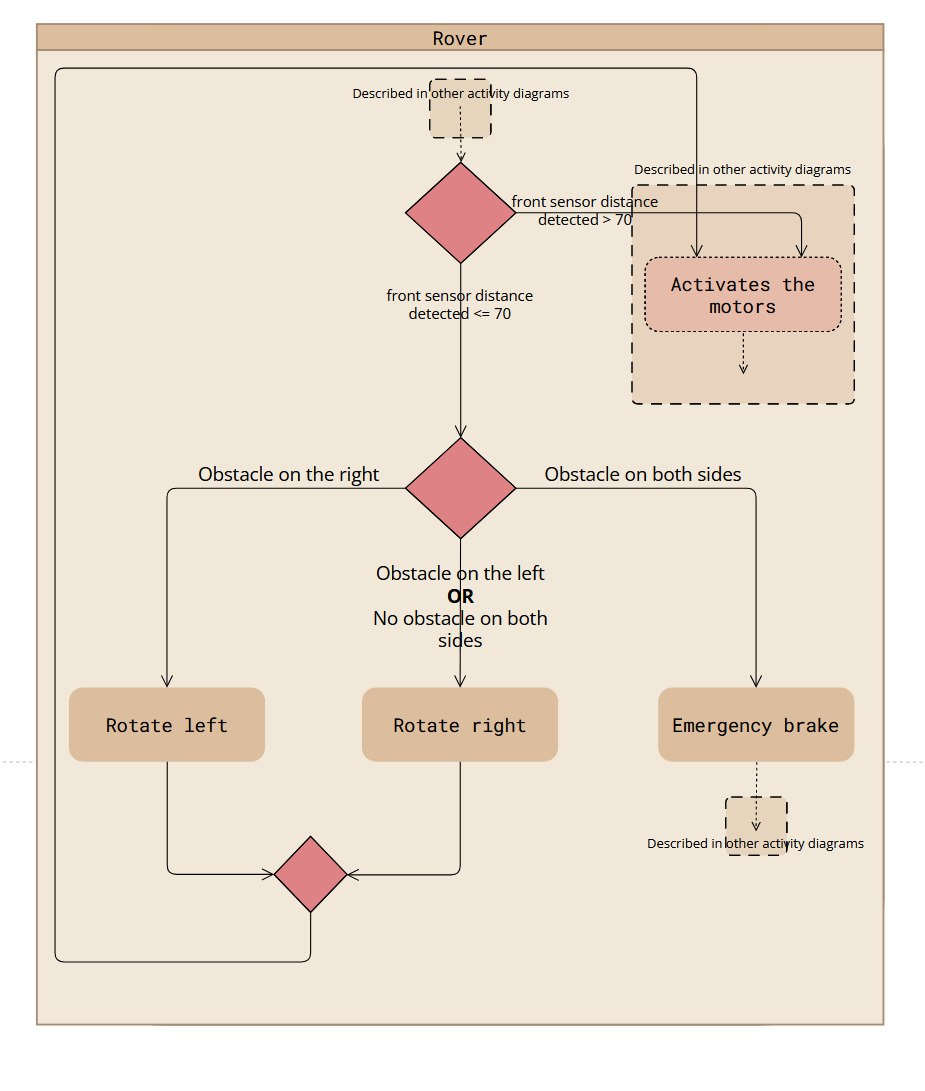
\includegraphics[width=0.7\linewidth]{../Use_Case_Diagram/Obstacle_Avoidance.jpg}
          \centering
          \caption{Obstacle Avoidance UML}
        \end{figure}
        Il processo inizia con il sensore frontale del rover che rileva un ostacolo. Se la distanza all’ostacolo è inferiore a 70 unità, attiva i motori. Se un ostacolo viene rilevato su entrambi i lati del rover, attiva un freno di emergenza. Se c’è un ostacolo solo da un lato (sia a sinistra che a destra), allora a seconda del lato in cui si trova l’ostacolo, ruota nella direzione opposta per evitarlo.

        \begin{itemize}
          \item \textbf{Sensori:}
          \begin{itemize}
              \item Rilevano ostacoli nelle vicinanze.
              \item Misurano la distanza agli ostacoli rilevati.
              \item Inviano segnali per attivare i motori o i freni di emergenza in base alla posizione e alla distanza dell'ostacolo.
          \end{itemize}
      
          \item \textbf{Rover:}
          \begin{itemize}
              \item Attiva i motori al ricevimento dei segnali dai sensori quando gli ostacoli sono vicini.
              \item Ruota a sinistra se rileva un ostacolo solo sul suo lato destro.
              \item Ruota a destra se rileva un ostacolo solo sul suo lato sinistro.
              \item Attiva i freni di emergenza se rileva ostacoli su entrambi i lati contemporaneamente.
          \end{itemize}
        \end{itemize}



      \subsubsection{Use Case Diagrams: Switch from Analog to Digital}
        \begin{figure}[h]
          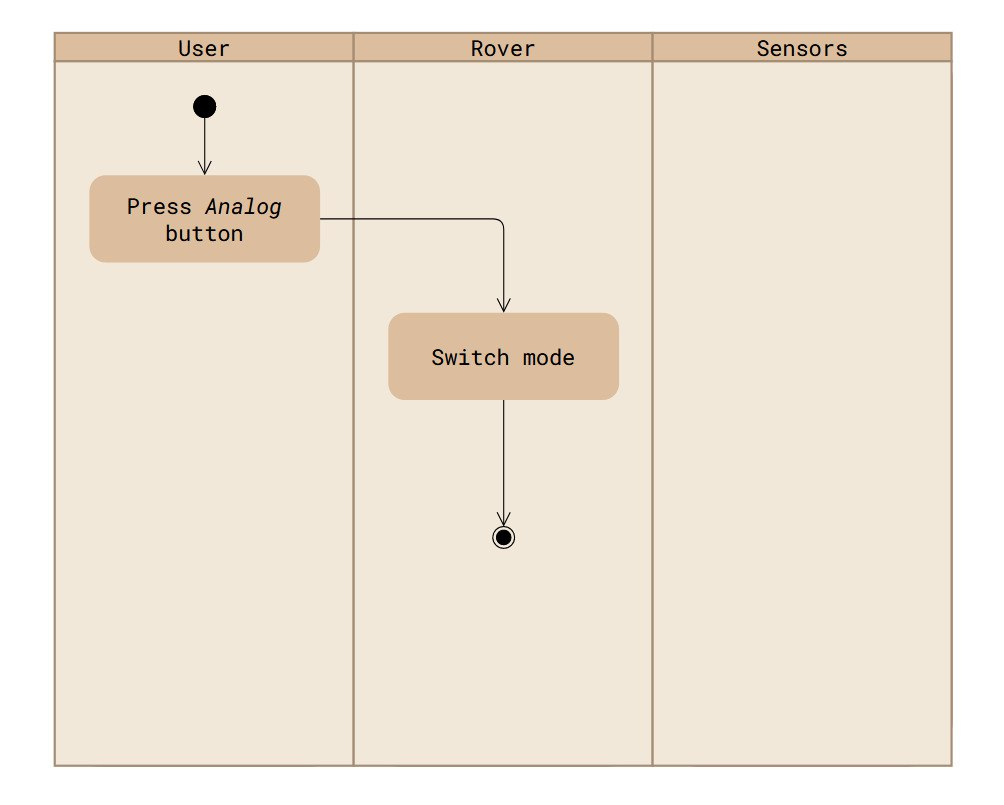
\includegraphics[width=0.7\linewidth]{../Use_Case_Diagram/Switch_Analog_To_Digital.jpg}
          \centering
          \caption{Mode Switch UML}       
        \end{figure}
        Il diagramma rappresenta il processo di passaggio da una modalità di comando digitale a una analogica. Il processo coinvolge l’utente che preme un pulsante analogico, che a sua volta attiva l’azione “Switch mode” nel rover.



      \subsubsection{Use Case Diagrams: Toggle Led}
        \begin{figure}[h]
          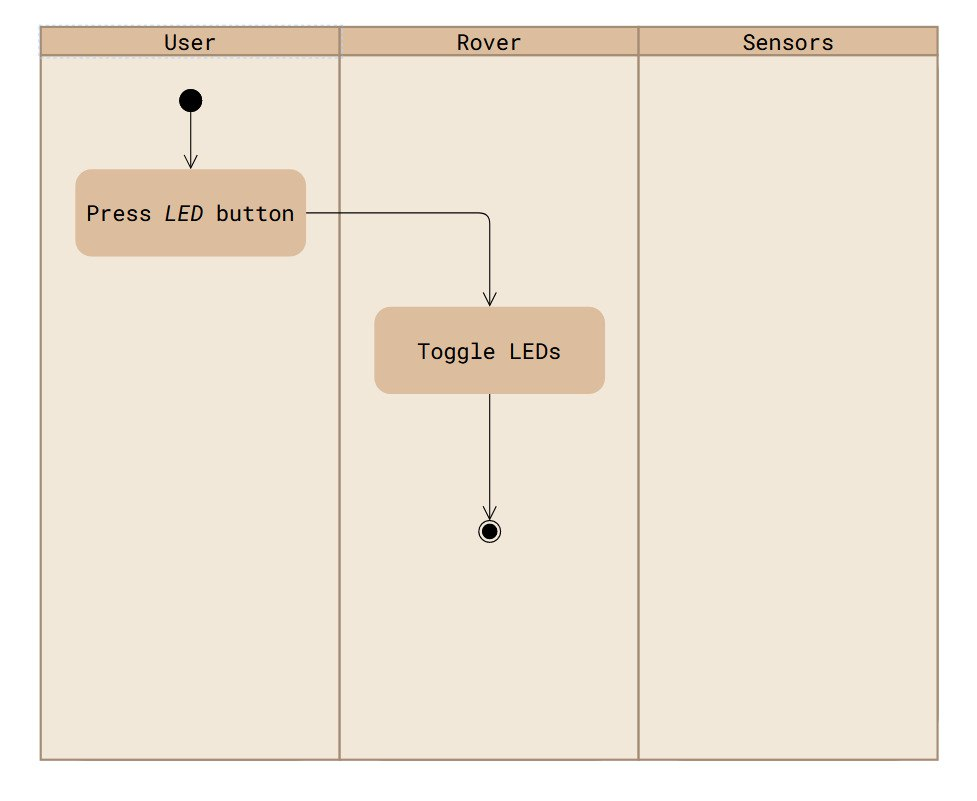
\includegraphics[width=0.7\linewidth]{../Use_Case_Diagram/Toggle_Led.jpg}
          \centering
          \caption{Toggle Led UML}     
        \end{figure}
        Similmente a prima, l'attivazione dei led è decretata dall'utente che preme un pulsante associato al toggle dei led: questo fa si che il rover, dal suo canto, proceda all'effettiva attivazione dei led. 



      \subsubsection{Use Case Diagrams: Turn On}
        \begin{figure}[h]
          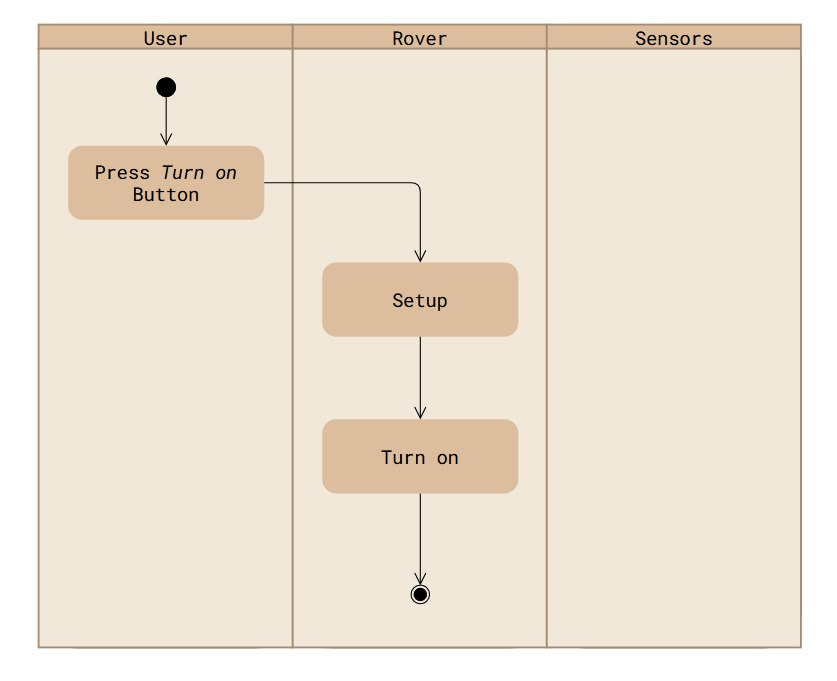
\includegraphics[width=0.7\linewidth]{../Use_Case_Diagram/Turn_on.jpg}
          \centering
          \caption{Turn On UML}
        \end{figure}
        Il diagramma rappresenta il processo di accensione di un rover. Il processo coinvolge l’utente che preme un pulsante di accensione, che a sua volta attiva l’azione “Setup” e poi “Turn on” nel rover. 












      \subsubsection{Sequence Diagrams}
      DA COMPLETARE DA COMPLETARE DA COMPLETARE
    \subsection{Timer}
        \subsubsection{Master}
          Il timer 1 è utilizzato contestualmente al sensore ad ultrasuoni centrale, in particolare viene impiegato per calcolare il tempo che trascorre tra i due fronti sul pin di echo. Per esso, è stato scelto un prescaler di 42-1 in modo tale da ottenere, unitamente ad una frequenza di clock di 42 MHz, una frequenza complessiva di 1MHz, ritenuta sufficiente per l'applicazione d'interesse. Concetti simili possono essere applicati per i timer 2 e per il timer 5, i quali però essendo entrambi associati ad un BUS a frequenza maggiore (84 MHz), hanno bisogno di essere prescalati di 84-1 per poter ottenere la frequenza di 1MHz precedentemente menzionata. 

          Per ogni timer è stata abilitata anche l'opzione di ricevere interruzione su fronte di salita o discesa del segnale sul pin di Echo, ovvero di ricezione dall'ultrasuono. 

          Infine, il TIM11 sebbene non esplicitamete selezionato, viene riservato (e dunque impiegato) come sorgente di SysTick e viene utilizzato dal framework di FreeRTOS. 

        \subsubsection{Slave} I timer 2, 3, 4 e 5 vengono utilizzati in Encoder Mode per poter determinare la velocità di crociera del rover. In questo caso il prescaler è stato impostato a 0, così che la frequenza complessiva non venisse edulcorata in alcun modo,  ottenendo una frequenza risultante di 84 MHz e dunque una maggiore precisione degli encoder. 

        Infine, il TIM11 sebbene non esplicitamete selezionato, viene riservato (e dunque impiegato) come sorgente di SysTick e viene utilizzato dal framework di FreeRTOS.


    \subsection{FreeRTOS}
    \subsection{Librerie prodotte}
        \subsubsection{Librerie Master}
          \paragraph{FreeRTOS\_Tasks} Questa libreria è stata creata per contenere in maniera atomica e indipendente tutti i task da schedulare, in modo da garantirvi un accesso più veloce e univoco. Questa libreria viene poi contestualmente richiamata all'interno della libreria \textit{freertos}. Per quanto riguarda una disamina dei task e delle motivazioni dietro la loro progettazione, si rimanda al capitolo 8.4. 
          \paragraph{panda\_comunication} L'argomento riveste una tale importanza che si è deciso di dedicare ad esso un manuale dedicato, presente sul Drive condiviso.
          \paragraph{panda\_hcsr04\_driver}
          Questo paragrafo ha lo scopo di illustrare brevemente, sulla base del funzionamento fisico del sensore descritto all'interno del volume I: hardware, le motivazione dietro la progettazione della libreria panda\_hcsr04\_driver. 

          Innanzitutto, si è voluto definire una struttura dati contenente tutta l'informazione utile al corretto funzionamento ed utilizzo del sensore, includendo inoltre una \textit{enum} al fine di racchiudere eventuali valori di ritorno possibili alle funzioni.

          Successivamente si è deciso di racchiudere l'attesa del pin di echo, insieme alla logica propria di utilizzo del dispositivo, all'interno della funzione \textit{panda\_HCSR04\_callback\_evaluations}, per poi utilizzare \textit{panda\_HCSR04\_get\_distance} per poter ottenere il valore effettivo della distanza. 

          Per poter correttamente contare il tempo utile al trigger output, è stata utilizzata una soluzione "alternativa" all'impiego del semplice SysTick, il quale non avrebbe consentito una risoluzione efficace per poter definire i microsecondi: si è dunque sperimentalmente verificato che una operazione di scrittura su pin impiegava circa 2.5 us, tale per cui ripeterne quattro avrebbe garantito i 10 us necessari. Questo avviene all'interno della funzione di \textit{reset}.  

          Si è scelto inoltre di associare lo stesso pin di trigger per tutti gli ultrasuoni, dovendo del resto utilizzarli contemporaneamente: dopo aver emesso il trigger, la scheda procede ad abilitare un timer per ciascun ultrasuono, che verra utilizzato poi per poter calcolare il tempo trascorso tra un fronte di salita e di discesa sul pin di Echo.

          E' bene notare che, a seguire del fronte sul pin associato al timer, l'IRQ viene gestita tramite una ISR esplicitata all'interno del file \textit{main.c}, ed essendo tutti i timer presenti sullo stesso APB (1, in particolare) la differenziazione tra i vari ultrasuoni viene fatta sulla base del parametro \textit{Istance} del timer associato all'interruzione. 


          \paragraph{panda\_motor\_driver} La progettazione della libreria ha dovuto chiaramente tenere conto del funzionamento stesso delle schede Sabertooth 2x12. Pertanto, si illustra brevemente il funzionamento dal punto di vista del protocollo dei dispositivi appena menzionati. 

          Al centro del funzionamento del Sabertooth 2X12 si trova la sua capacità di ricevere comandi da una varietà di fonti e di tradurli in movimenti del motore. Questi comandi possono provenire da un segnale analogico, da un segnale di controllo radio (R/C), o da un flusso di dati seriali. Questa flessibilità nel ricevere comandi da diverse fonti rende il Sabertooth 2X12 adatto a una vasta gamma di applicazioni. Ad esempio, in un’applicazione robotica come quella d'interesse, si è utilzzato un segnale sia analogico che digitale da un controller ps2 per regolare il movimento del robot.

          Nel caso del controllo seriale, il Sabertooth 2X12 può operare in due modalità: seriale semplificata e seriale pacchettizzata. In entrambe le modalità, i comandi vengono inviati al Sabertooth 2X12 come flusso di dati a livello TTL (Transistor-Transistor Logic) collegato al terminale S1 del dispositivo. La logica TTL è un tipo di logica digitale che utilizza transistor per implementare le porte logiche. È ampiamente utilizzata nei circuiti digitali a causa della sua robustezza e della sua capacità di operare a velocità relativamente elevate. Il fatto che il Sabertooth 2X12 utilizzi la logica TTL per la sua interfaccia seriale significa che può essere facilmente interfacciato con una vasta gamma di dispositivi, tra cui la maggior parte dei microcontrollori e dei computer.

          Nella modalità seriale semplificata, il controllo è effettuato tramite comandi di un singolo byte. Per esempio, per il motore 1, un valore di 1 corrisponde a piena retromarcia, 64 corrisponde a stop, e 127 corrisponde a piena marcia avanti. Analogamente, per il motore 2, un valore di 128 corrisponde a piena retromarcia, 192 corrisponde a stop, e 255 corrisponde a piena marcia avanti. Questa modalità offre un modo semplice e diretto per controllare i motori. Tuttavia, la sua semplicità ha un costo in termini di precisione e flessibilità. Ad esempio, in questa modalità, la velocità dei motori può essere controllata solo in 128 passi da piena retromarcia a piena marcia avanti. Inoltre, in questa modalità, non è possibile indirizzare più dispositivi Sabertooth sulla stessa linea seriale.

          Nella modalità seriale pacchettizzata, i comandi sono inviati come un pacchetto di più byte. Questa modalità offre un controllo più fine e la possibilità di indirizzare più dispositivi Sabertooth sulla stessa linea seriale. In questa modalità, ogni comando è composto da un byte di indirizzo, un byte di comando e un byte di dati, seguiti da un byte di checksum per la verifica degli errori. Questo formato di comando permette di controllare fino a 128 dispositivi Sabertooth sulla stessa linea seriale, ognuno con 128 livelli di velocità da piena retromarcia a piena marcia avanti. Inoltre, questa modalità offre una maggiore robustezza rispetto alla modalità seriale semplificata, grazie all’uso del checksum per la verifica degli errori.

          In entrambe le modalità, i comandi inviati al Sabertooth 2X12 determinano la velocità e la direzione dei motori collegati al dispositivo. Questo permette di controllare con precisione il movimento del robot o del veicolo radiocomandato. Ad esempio, inviando un comando di “piena marcia avanti” al motore 1 e un comando di “stop” al motore 2, è possibile far girare il robot o il veicolo a destra. Inviando un comando di “piena marcia avanti” a entrambi i motori, è possibile far avanzare il robot o il veicolo dritto. Inviando comandi di “piena retromarcia” a entrambi i motori, è possibile far indietreggiare il robot o il veicolo. 

          Avendo chiaro il funzionamento logico, è possibile procedere ad illustrare la progettazione della libreria utile ad interagire con le Sabertooth 2x12. 

          Innanzitutto, si è scelto di utilizzare la modalità pacchettizzata, sulla base dei vantaggi precedentemente illustrati, che risultavano quasi scelta obbligata nel contesto del progetto, stanti le specifiche da soddisfare, in particolare stante la volontà di ridurre il numero di cavi presenti tra Sabertooth e schede STM. Chiaramente, per poter sfrutturare questa possibilità, si è dovuto utilizzare un indirizzo associato a ciascuna Sabertooth, impostato attivando un apposito switch presente sul dispositivo. 

          Inoltre, altro accorgimento messo in atto, è stato quello di istruire le Sabertooth ad utilizzare un Baud Rate che fosse il massimo possibile, ovvero 38400. Per fare ciò, attraverso un ciclo for aumentante di 100 in 100, si è fatto numerosi tentativi d'invio del comando finchè non si è riusciti ad impartire il Baud Rate desiderato: questo è stato fatto al fine di avere una comunicazione con i dispositivi che fosse il più rapida possibile. 

          Per poter garantire anche la possibilità di svolta in movimento, si è optato per una modalità \textit{mixed} di invio dei comandi, che permette di controllare due motori contemporaneamente: sulla base di questa logica implementativa, si è allora scelto di realizzare funzioni per la svolta a destra, a sinistra, o per la retromarcia. 

          In aggiunta, si è implementato anche il checksum messo a disposizione dai dispositivi (contestuale alla comunicazione dei comandi dalle schede STM alle Sabertooth) definito come segue: nella modalità seriale pacchettizzata, ogni comando inviato al Sabertooth 2X12 è composto da un byte di indirizzo, un byte di comando, un byte di dati e un byte di checksum. Il byte di checksum è calcolato sommando il byte di indirizzo, il byte di comando e il byte di dati, e poi prendendo il modulo 128 del risultato1. Questo significa che il byte di checksum è il resto della divisione della somma dei primi tre byte per 128. Il byte di checksum viene quindi inviato al Sabertooth 2X12 insieme ai primi tre byte. Quando il Sabertooth 2X12 riceve un comando, calcola il checksum in modo simile, sommando il byte di indirizzo, il byte di comando e il byte di dati ricevuti, e prendendo il modulo 128 del risultato. Quindi confronta il checksum calcolato con il byte di checksum ricevuto. Se i due checksum corrispondono, il Sabertooth 2X12 accetta il comando come valido. Se i due checksum non corrispondono, il Sabertooth 2X12 rifiuta il comando come non valido.

          Come già accennato, per ciascun comando impartibile è stata definita una funzione, ed è stata inoltre definita una funzione "cappello" con lo scopo di creare i comandi veri e propri sulla base di un numerico associato al comando e sul valore relativo. Questa funzione inoltre si occupa di definire il checksum e inviare tramite UART il comando. 


          \paragraph{panda\_mpu6050} Questo codice è progettato per interfacciarsi con il sensore \textit{MPU6050}, un sensore di movimento a 6 assi che include un accelerometro e un giroscopio. La libreria \textit{panda\_mpu6050} fornisce un’interfaccia di alto livello per interagire con questo sensore.

          La funzione \textit{panda\_mpu6050\_init} inizializza la struttura dati \textit{MPU6050\_t} che contiene tutte le informazioni necessarie per interagire con il sensore. Questa funzione imposta tutti i valori iniziali a zero, che è una buona pratica per evitare comportamenti imprevisti dovuti a dati non inizializzati.
          
          Successivamente, la funzione legge il registro \textit{WHO\_AM\_I} del sensore per verificare che la comunicazione I2C sia stata stabilita correttamente. Se il valore letto è 104, che è il valore atteso per il sensore MPU6050, allora la funzione procede con la configurazione del sensore. Altrimenti, restituisce un errore.
          
          La configurazione del sensore include l’impostazione del registro \textit{PWR\_MGMT\_1} a zero per svegliare il sensore, l’impostazione del registro \textit{SMPLRT\_DIV} a 0x07 per impostare la frequenza di campionamento, e l’impostazione dei registri \textit{ACCEL\_CONFIG} e \textit{GYRO\_CONFIG} a zero per configurare l’accelerometro e il giroscopio con la massima risoluzione e il range di misura.
          
          La funzione \textit{panda\_mpu6050\_read} legge i dati dal sensore. Prima legge i dati grezzi da tutti i registri del sensore, poi converte questi dati grezzi in valori utilizzabili. Ad esempio, divide i dati grezzi dell’accelerometro per $16384.0$ per convertirli in g, e divide i dati grezzi del giroscopio per $131.0$ per convertirli in gradi al secondo. Infine, calcola la temperatura del sensore utilizzando la formula fornita nel datasheet del sensore.
          
          
          \paragraph{panda\_psx\_controller}
          La funzione panda\_psx\_init inizializza il controller PSX. Questa funzione prende come parametri una struttura psx\_t (che contiene le informazioni del controller), un SPI\_HandleTypeDef (che gestisce la comunicazione SPI), un GPIO\_TypeDef (che gestisce la porta GPIO) e un uint16\_t (che gestisce il pin GPIO). Questa funzione configura il controller per l’uso e restituisce PSX\_OK se l’inizializzazione ha avuto successo. Questa funzione è simile alla funzione config\_gamepad della libreria Arduino\-PS2X, che inizializza il controller PSX specificando i pin a cui è collegato il controller e le opzioni per abilitare la vibrazione e la lettura delle pressioni dei pulsanti.

          La funzione panda\_psx\_read\_gamepad legge lo stato del gamepad. Invia un array di byte al controller PSX tramite SPI e riceve lo stato del gamepad. Se la trasmissione e la ricezione hanno successo, la funzione restituisce PSX\_OK; altrimenti, restituisce PSX\_ERROR. Questa funzione è simile alla funzione read\_gamepad della libreria Arduino\-PS2X, che legge lo stato del gamepad inviando un array di byte al controller PSX tramite SPI e ricevendo lo stato del gamepad.
          
          La funzione panda\_psx\_get\_command ottiene un comando dal controller. Prende come parametri una struttura psx\_t e un PSX\_ButtonsTypeDef che indica il pulsante da leggere. Questa funzione restituisce lo stato del pulsante. Questa funzione è simile alla funzione Button della libreria Arduino\-PS2X, che ottiene lo stato di un pulsante del controller.
          
          La funzione panda\_psx\_get\_analog\_intensity ottiene l’intensità analogica di un asse del controller. Prende come parametri una struttura psx\_t e un PSX\_AnalogTypeDef che indica l’asse da leggere. Questa funzione restituisce l’intensità analogica dell’asse. Questa funzione è simile alla funzione Analog della libreria Arduino\-PS2X, che ottiene l’intensità analogica di un asse del controller.
        \subsubsection{Librerie Slave}
          \paragraph{FreeRTOS\_Tasks} Quanto detto per l'omonima libreria presente sulla scheda Master varrà anche in questo caso: difatti, si rimanda al capitolo 8.4 per ulteriori informazioni circa i task previsti. 
          \paragraph{panda\_comunication} L'argomento riveste una tale importanza che si è deciso di dedicare ad esso manuale a parte presente sul Drive condiviso. 
          \paragraph{panda\_motor\_driver} La libreria risulta esattamente identica a quella prevista per il master.
  \section{Implementazione}
    In questo capitolo si illustrerà il codice prodotto contestualmente alle varie librerie. 
    \subsection{ADC}
        \subsubsection{Master$>$adc.h}
          Iniziamo con le direttive del preprocessore \texttt{\#ifndef \_\_ADC\_H\_\_} e \texttt{\#endif}. Queste impediscono l'inclusione multipla del file di intestazione nel codice sorgente, un concetto noto come "inclusione protettiva". Questo è importante perché l'inclusione multipla dello stesso file di intestazione può causare problemi di compilazione.

          Le linee \texttt{\#ifdef \_\_cplusplus} e \texttt{extern "C"} sono usate per garantire la compatibilità con il codice C++ nel caso in cui questo file di intestazione venga incluso in un file sorgente C++. Questo è utile se stai lavorando in un ambiente di sviluppo misto C/C++.
          
          Il file include anche il file "main.h" con \texttt{\#include "main.h"}. Questo file "main.h" probabilmente contiene definizioni e dichiarazioni globali che vengono utilizzate in tutto il progetto.
          
          La linea \texttt{extern ADC\_HandleTypeDef hadc1;} dichiara \texttt{hadc1} come una variabile esterna. \texttt{ADC\_HandleTypeDef} è probabilmente un tipo definito dall'utente, molto probabilmente una struttura, che contiene informazioni relative alla configurazione e allo stato del convertitore ADC sulla tua scheda STM32F401RE.
          
          Infine c'è ovviamente la dichiarazione di una funzione \texttt{void MX\_ADC1\_Init(void);}. Questa funzione sarà utilizzata per preparare l'ADC a leggere i sensori di batteria e temperatura.
        \subsubsection{Master$>$adc.c}
        Il codice in esame è utilizzato per la configurazione e l'inizializzazione di un modulo ADC (Analog to Digital Converter) su una scheda STM32F401RE. Questo ADC viene utilizzato per leggere i sensori di batteria e temperatura.

        Il codice inizia con l'inclusione del file di intestazione "adc.h", che contiene le dichiarazioni delle funzioni e le definizioni dei tipi utilizzati nel file sorgente.
        
        \begin{lstlisting}[style=CStyle]
        #include "adc.h"
        \end{lstlisting}
        
        Successivamente, viene definita una variabile globale `hadc1` di tipo `ADC\_HandleTypeDef`. Questa struttura gestisce le configurazioni e lo stato dell'ADC.
        
        \begin{lstlisting}[style=CStyle]
        ADC_HandleTypeDef hadc1;
        \end{lstlisting}
        
        La funzione `MX\_ADC1\_Init` è responsabile dell'inizializzazione dell'ADC. Configura le caratteristiche globali dell'ADC come il prescaler dell'orologio, la risoluzione, la modalità di conversione, il trigger esterno, l'allineamento dei dati e il numero di conversioni. Inoltre, configura il canale ADC selezionato, il suo rango nella sequenza e il suo tempo di campionamento.
        
        \begin{lstlisting}[style=CStyle]
        void MX\_ADC1\_Init(void)
        {
          ADC\_ChannelConfTypeDef sConfig = {0};
        
          hadc1.Instance = ADC1;
          hadc1.Init.ClockPrescaler = ADC_CLOCK_SYNC_PCLK_DIV2;
          hadc1.Init.Resolution = ADC_RESOLUTION_12B;
          hadc1.Init.ScanConvMode = DISABLE;
          hadc1.Init.ContinuousConvMode = ENABLE;
          hadc1.Init.DiscontinuousConvMode = DISABLE;
          hadc1.Init.ExternalTrigConvEdge = ADC_EXTERNALTRIGCONVEDGE_NONE;
          hadc1.Init.ExternalTrigConv = ADC_SOFTWARE_START;
          hadc1.Init.DataAlign = ADC_DATAALIGN_RIGHT;
          hadc1.Init.NbrOfConversion = 1;
          hadc1.Init.DMAContinuousRequests = DISABLE;
          hadc1.Init.EOCSelection = ADC_EOC_SEQ_CONV;
          if (HAL_ADC_Init(&hadc1) != HAL_OK)
          {
            Error_Handler();
          }
        
          sConfig.Channel = ADC_CHANNEL_TEMPSENSOR;
          sConfig.Rank = 1;
          sConfig.SamplingTime = ADC_SAMPLETIME_3CYCLES;
          if (HAL_ADC_ConfigChannel(&hadc1, &sConfig) != HAL_OK)
          {
            Error_Handler();
          }
        }
        \end{lstlisting}
        
        Le funzioni `HAL\_ADC\_MspInit` e `HAL\_ADC\_MspDeInit` sono funzioni di callback che vengono chiamate quando l'ADC viene rispettivamente inizializzato e de-inizializzato. Queste funzioni configurano i pin GPIO utilizzati dall'ADC e abilitano o disabilitano l'orologio periferico dell'ADC.
        
        \begin{lstlisting}[style=CStyle]
        void HAL_ADC_MspInit(ADC_HandleTypeDef* adcHandle)
        {
          GPIO_InitTypeDef GPIO_InitStruct = {0};
          if(adcHandle->Instance==ADC1)
          {
            __HAL_RCC_ADC1_CLK_ENABLE();
        
            __HAL_RCC_GPIOA_CLK_ENABLE();
            GPIO_InitStruct.Pin = Battery_Sensor_ADC_Pin;
            GPIO_InitStruct.Mode = GPIO_MODE_ANALOG;
            GPIO_InitStruct.Pull = GPIO_NOPULL;
            HAL_GPIO_Init(Battery_Sensor_ADC_GPIO_Port, &GPIO_InitStruct);
          }
        }
        
        void HAL_ADC_MspDeInit(ADC_HandleTypeDef* adcHandle)
        {
          if(adcHandle->Instance==ADC1)
          {
            __HAL_RCC_ADC1_CLK_DISABLE();
            HAL_GPIO_DeInit(Battery_Sensor_ADC_GPIO_Port, Battery_Sensor_ADC_Pin);
          }
        }
        \end{lstlisting}
    \subsection{Master$>$led.h}
        All'interno di questo file è presente soltanto una \textit{enum} utile a definire univocamente i possibili stati dei led. 
    \subsection{Master$>$main.h}
        
      Il file inizia con alcune direttive del preprocessore per prevenire l'inclusione ricorsiva, che potrebbe causare problemi di compilazione. Inoltre, verifica se il codice viene compilato come C++ e, in caso affermativo, avvolge le dichiarazioni in un blocco `extern "C"` per garantire la compatibilità con il codice C++.

      \begin{lstlisting}[style=CStyle]
      /* Define to prevent recursive inclusion -------------------------------------*/
      #ifndef __MAIN_H
      #define __MAIN_H

      #ifdef __cplusplus
      extern "C" {
      #endif
      \end{lstlisting}

      Successivamente, il file include l'header "stm32f4xx\_hal.h", che contiene le definizioni e le dichiarazioni per l'Hardware Abstraction Layer (HAL) per STM32F4xx.

      \begin{lstlisting}[style=CStyle]
      /* Includes ------------------------------------------------------------------*/
      #include "stm32f4xx_hal.h"
      \end{lstlisting}

      Il file definisce anche una macro `VERBOSE` con il valore 0. Questa macro può essere utilizzata nel codice per abilitare o disabilitare la stampa di messaggi di debug.

      \begin{lstlisting}[style=CStyle]
      /* Exported constants --------------------------------------------------------*/
      /* USER CODE BEGIN EC */
      #define VERBOSE 0
      /* USER CODE END EC */
      \end{lstlisting}

      Il file dichiara due funzioni, `Error\_Handler` e `Global\_Struct\_Master\_Init`. Queste funzioni sono dichiarate ma non definite in questo file, quindi le loro definizioni devono essere presenti in un altro file sorgente.

      \begin{lstlisting}[style=CStyle]
      /* Exported functions prototypes ---------------------------------------------*/
      void Error_Handler(void);

      /* USER CODE BEGIN EFP */
      void Global_Struct_Master_Init();
      /* USER CODE END EFP */
      \end{lstlisting}

      Infine, il file definisce una serie di macro per i pin GPIO e le porte utilizzate nel progetto. Queste macro vengono utilizzate per riferirsi ai pin specifici sulla scheda STM32F401RE.

      \begin{lstlisting}[style=CStyle]
      /* Private defines -----------------------------------------------------------*/
      #define Sync_Input_Pin GPIO_PIN_2
      #define Sync_Input_GPIO_Port GPIOC
      #define Sync_Output_Pin GPIO_PIN_3
      #define Sync_Output_GPIO_Port GPIOC
      #define Battery_Sensor_ADC_Pin GPIO_PIN_0
      #define Battery_Sensor_ADC_GPIO_Port GPIOA
      #define UltraSound3_RX_Pin GPIO_PIN_1
      #define UltraSound3_RX_GPIO_Port GPIOA
      #define PSX_SCK_Pin GPIO_PIN_5
      #define PSX_SCK_GPIO_Port GPIOA
      #define PSX_MISO_Pin GPIO_PIN_6
      #define PSX_MISO_GPIO_Port GPIOA
      #define PSX_MOSI_Pin GPIO_PIN_7
      #define PSX_MOSI_GPIO_Port GPIOA
      #define PSX_Att_Pin GPIO_PIN_8
      #define PSX_Att_GPIO_Port GPIOC
      #define Accelerometer_SDA_Pin GPIO_PIN_9
      #define Accelerometer_SDA_GPIO_Port GPIOC
      #define Accelerometer_SCL_Pin GPIO_PIN_8
      #define Accelerometer_SCL_GPIO_Port GPIOA
      #define UltraSound1_RX_Pin GPIO_PIN_9
      #define UltraSound1_RX_GPIO_Port GPIOA
      #define Turn_Off_Slave_Pin GPIO_PIN_10
      #define Turn_Off_Slave_GPIO_Port GPIOC
      #define UltraSound2_RX_Pin GPIO_PIN_3
      #define UltraSound2_RX_GPIO_Port GPIOB
      #define MotorDriver_TX_Pin GPIO_PIN_6
      #define MotorDriver_TX_GPIO_Port GPIOB
      #define Comunication_SDA_Pin GPIO_PIN_7
      #define Comunication_SDA_GPIO_Port GPIOB
      #define Comunication_SCL_Pin GPIO_PIN_8
      #define Comunication_SCL_GPIO_Port GPIOB
      #define Ultrasound_Trigger_Pin GPIO_PIN_9
      #define Ultrasound_Trigger_GPIO_Port GPIOB
      \end{lstlisting}

    \subsection{Master$>$main.c}
    \subsection{Master$>$panda\_hcsr04\_driver.h}
    \begin{lstlisting}[style=CStyle]
      /**
        ******************************************************************************
        * @file panda_hcsr04_driver.h
        * @brief This file contains all the functions prototypes for the panda_hcsr04_driver.c file.
        *
        * It provides an interface for interacting with the HCSR04 ultrasonic sensor module.
        *
        * It includes the necessary structures, enumerations, and function prototypes to initialize and read the HCSR04 Module.
        * It provides a convenient and structured way to retrieve information from the module.
        *
        *
        *
        ******************************************************************************
        *
        * Copyright (c) 2023 STMicroelectronics.
        * All rights reserved.
        *
        * This software is licensed under terms that can be found in the LICENSE file
        * in the root directory of this software component.
        * If no LICENSE file comes with this software, it is provided AS-IS.
        *
        ******************************************************************************
        */
      #ifndef INC_PANDA_HCSR04_DRIVER_H_
      #define INC_PANDA_HCSR04_DRIVER_H_
      \end{lstlisting}
      
      Il file inizia con un commento di intestazione che fornisce informazioni sul file, come il nome del file, la sua funzione principale e le informazioni sul copyright.
      
      Successivamente, il file include un file di intestazione e definisce una macro per il pin del trigger. Questi sono utilizzati per configurare l'interfaccia GPIO per il modulo del sensore ad ultrasuoni HCSR04.
      
      \begin{lstlisting}[style=CStyle]
      #include <stdint.h>
      #include "gpio.h"
      
      #define Trigger_Pin GPIO_PIN_9
      #define Trigger_GPIO_Port GPIOB
      \end{lstlisting}
      
      Il file definisce un'enumerazione per lo stato del modulo HCSR04 e una struttura per i dati del modulo HCSR04. Questi vengono utilizzati per gestire lo stato del modulo e per memorizzare i dati rilevati dal modulo.
      
      \begin{lstlisting}[style=CStyle]
      /**
       * @brief Enumeration for the HCSR04 module status.
       */
      typedef enum{
        HCSR04_OK = 0, /**< OK status */
        HCSR04_ERR = 1 /**< Error status */
      }HCSR04_StatusTypeDef;
      
      
      /**
       * @brief Structure for the HCSR04 module data.
       */
      typedef struct{
        GPIO_TypeDef* port_trigger;
        uint16_t pin_trigger;
        GPIO_TypeDef* port_echo;
        uint16_t pin_echo;
        TIM_HandleTypeDef* timer;
      
        uint32_t IC_Val1;
        uint32_t IC_Val2;
        uint32_t Difference;
        uint8_t Is_First_Captured;
        uint16_t Distance;
      }HCSR04_t;
      \end{lstlisting}
      
      Il file dichiara una serie di funzioni per interagire con il modulo del sensore ad ultrasuoni HCSR04. Queste funzioni includono l'inizializzazione del modulo, la valutazione dei callback dal modulo, il reset del modulo e la lettura della distanza misurata dal modulo.
      
      \begin{lstlisting}[style=CStyle]
      /**
       * @brief Initializes the HCSR04 ultrasonic sensor.
       *
       * This function initializes the HCSR04 ultrasonic sensor by setting up the timer handle, GPIO port and pin for the trigger signal. It also initializes the internal variables of the HCSR04 structure.
       *
       * @param ultrasound Pointer to the HCSR04 structure.
       * @param timer Pointer to the timer handle.
       * @param port_trigger Pointer to the GPIO port used for the trigger signal.
       * @param pin_trigger The pin number used for the trigger signal.
       * @return HCSR04_StatusTypeDef Returns HCSR04_OK after successful initialization.
       */
      HCSR04_StatusTypeDef panda_HCSR04_init(HCSR04_t* ultrasound, TIM_HandleTypeDef *timer, GPIO_TypeDef* port_trigger, uint16_t pin_trigger);
      
      
      /**
       * @brief Evaluates the callback from the HCSR04 ultrasonic sensor.
       *
       * This function evaluates the callback from the HCSR04 ultrasonic sensor by reading the captured values from the timer and calculating the distance based on these values.
       *
       * @param ultrasound Pointer to the HCSR04 structure.
       * @param Channel The timer channel.
       * @return HCSR04_StatusTypeDef Returns HCSR04_OK if the callback was successfully evaluated, or HCSR04_ERROR if there was an error.
       */
      HCSR04_StatusTypeDef panda_HCSR04_callback_evaluations(HCSR04_t* ultrasound, uint32_t Channel);
      
      /**
       * @brief Resets the HCSR04 ultrasonic sensors.
       *
       * This function resets the HCSR04 ultrasonic sensors by setting the trigger pin to high and then to low, and enabling the timer interrupt.
       *
       * @param ultrasound_left Pointer to the left HCSR04 structure.
       * @param ultrasound_middle Pointer to the middle HCSR04 structure.
       * @param ultrasound_right Pointer to the right HCSR04 structure.
       * @return HCSR04_StatusTypeDef Returns HCSR04_OK after successful reset.
       */
      HCSR04_StatusTypeDef panda_HCSR04_reset(HCSR04_t* ultrasound_left, HCSR04_t* ultrasound_middle, HCSR04_t* ultrasound_right);
      
      /**
       * @brief Gets the distance measured by the HCSR04 ultrasonic sensor.
       *
       * This function gets the distance measured by the HCSR04 ultrasonic sensor. If the sensor is still capturing, it returns a default value of 999.
       *
       * @param ultrasound Pointer to the HCSR04 structure.
       * @return uint16_t Returns the distance measured by the sensor, or 999 if the sensor is still capturing.
       */
      uint16_t panda_HCSR04_get_distance(HCSR04_t* ultrasound);
      #endif /* INC_PANDA_HCSR04_DRIVER_H_ */
      \end{lstlisting}      
    \subsection{Master$>$panda\_hcsr04\_driver.c}
    \begin{lstlisting}[style=CStyle]
      #include "panda_hcsr04_driver.h"
      #include "stm32f4xx_hal.h"
      #include "tim.h"
      #include "gpio.h"
      #include <stdint.h>
      #include <stdio.h>
      \end{lstlisting}
      
      Queste righe includono i file di intestazione necessari per il tuo programma. Questi file di intestazione forniscono le definizioni e le dichiarazioni per vari aspetti del tuo programma, come le funzioni del driver del sensore ad ultrasuoni HCSR04, le funzioni HAL per la scheda STM32F4xx, le funzioni per i timer, le funzioni per l'interfaccia GPIO, e le librerie standard per i tipi di dati interi e le funzioni di input/output.
      
      \begin{lstlisting}[style=CStyle]
      HCSR04_StatusTypeDef panda_HCSR04_init(HCSR04_t* ultrasound, TIM_HandleTypeDef *timer, GPIO_TypeDef* port_trigger, uint16_t pin_trigger){
      \end{lstlisting}
      
      Questa riga definisce la funzione `panda\_HCSR04\_init`, che inizializza il sensore ad ultrasuoni HCSR04. La funzione prende come argomenti un puntatore alla struttura `HCSR04\_t` (che rappresenta il sensore ad ultrasuoni), un puntatore alla struttura `TIM\_HandleTypeDef` (che rappresenta il timer utilizzato per misurare il tempo di ritorno del segnale ad ultrasuoni), un puntatore alla struttura `GPIO\_TypeDef` (che rappresenta la porta GPIO utilizzata per il segnale di trigger), e un intero senza segno a 16 bit (che rappresenta il pin utilizzato per il segnale di trigger).
      
      \begin{lstlisting}[style=CStyle]
        int8_t res = HCSR04_ERR;
      
        ultrasound->port_trigger = port_trigger;
        ultrasound->pin_trigger = pin_trigger;
        ultrasound->timer = timer;
        ultrasound->IC_Val1 =  0;
        ultrasound->IC_Val2 = 0;
        ultrasound->Difference =0;
        ultrasound->Is_First_Captured = 0;
        ultrasound->Distance = 0;
      
        res = HCSR04_OK;
      
        return res;
      \end{lstlisting}
      
      All'interno della funzione `panda\_HCSR04\_init`, viene inizialmente impostata una variabile `res` con il valore `HCSR04\_ERR`. Successivamente, vengono impostati i campi della struttura `ultrasound` con i valori passati come argomenti alla funzione e vengono inizializzati altri campi della struttura `ultrasound` a zero. Infine, la variabile `res` viene impostata su `HCSR04\_OK` e restituita dalla funzione, indicando che l'inizializzazione è stata eseguita correttamente.
      
      \begin{lstlisting}[style=CStyle]
      HCSR04_StatusTypeDef panda_HCSR04_callback_evaluations(HCSR04_t* ultrasound, uint32_t Channel){
      \end{lstlisting}
      
      Questa riga definisce la funzione `panda\_HCSR04\_callback\_evaluations`, che valuta il callback dal sensore ad ultrasuoni HCSR04. La funzione prende come argomenti un puntatore alla struttura `HCSR04\_t` (che rappresenta il sensore ad ultrasuoni) e un intero senza segno a 32 bit (che rappresenta il canale del timer).
      
      \begin{lstlisting}[style=CStyle]
        uint8_t res = HCSR04_ERR;
      
        if (ultrasound->Is_First_Captured==0)
        {
          ultrasound->IC_Val1 = HAL_TIM_ReadCapturedValue(ultrasound->timer, Channel);
          ultrasound->Is_First_Captured = 1;
          __HAL_TIM_SET_CAPTUREPOLARITY(ultrasound->timer, Channel, TIM_INPUTCHANNELPOLARITY_FALLING);
        }
      
        else if (ultrasound->Is_First_Captured==1)
        {
          ultrasound->IC_Val2 = HAL_TIM_ReadCapturedValue(ultrasound->timer, Channel);
          __HAL_TIM_SET_COUNTER(ultrasound->timer, 0);
      
          if (ultrasound->IC_Val2 > ultrasound->IC_Val1)
          {
            ultrasound->Difference = ultrasound->IC_Val2-ultrasound->IC_Val1;
          }
      
          else if (ultrasound->IC_Val1 > ultrasound->IC_Val2)
          {
            ultrasound->Difference = (0xffff - ultrasound->IC_Val1) + ultrasound->IC_Val2;
          }
          ultrasound->Distance = ultrasound->Difference *0.017;
      
          ultrasound->Is_First_Captured = 0;
      
          __HAL_TIM_SET_CAPTUREPOLARITY(ultrasound->timer, Channel, TIM_INPUTCHANNELPOLARITY_RISING);
      
      
          res = HCSR04_OK;
        }
        return res;
      \end{lstlisting}
      
      All'interno della funzione `panda\_HCSR04\_callback\_evaluations`, viene inizialmente impostata una variabile `res` con il valore `HCSR04\_ERR`. Successivamente, la funzione controlla se è la prima volta che viene catturato un valore. Se è così, legge il valore catturato dal timer, lo salva nel campo `IC\_Val1` della struttura `ultrasound`, imposta il campo `Is\_First\_Captured` a 1 e cambia la polarità di cattura del timer a `TIM\_INPUTCHANNELPOLARITY\_FALLING`. Se non è la prima volta che viene catturato un valore, la funzione legge nuovamente il valore catturato dal timer, lo salva nel campo `IC\_Val2` della struttura `ultrasound`, azzera il contatore del timer e calcola la differenza tra `IC\_Val2` e `IC\_Val1`. Questa differenza viene poi utilizzata per calcolare la distanza. Infine, la funzione reimposta il campo `Is\_First\_Captured` a 0, cambia la polarità di cattura del timer a `TIM\_INPUTCHANNELPOLARITY\_RISING` e imposta la variabile `res` a `HCSR04\_OK`. La variabile `res` viene quindi restituita dalla funzione.
      
      \begin{lstlisting}[style=CStyle]
      HCSR04_StatusTypeDef panda_HCSR04_reset(HCSR04_t* ultrasound_left, HCSR04_t* ultrasound_middle, HCSR04_t* ultrasound_right){
      \end{lstlisting}
      
      Questa riga definisce la funzione `panda\_HCSR04\_reset`, che resetta i sensori ad ultrasuoni HCSR04. La funzione prende come argomenti tre puntatori alle strutture `HCSR04\_t` (che rappresentano i sensori ad ultrasuoni sinistro, centrale e destro).
      
      \begin{lstlisting}[style=CStyle]
        uint8_t res = HCSR04_ERR;
      
        for(int i = 0; i<4; i++) HAL_GPIO_WritePin(ultrasound_left->port_trigger, ultrasound_left->pin_trigger, GPIO_PIN_SET);
      
        HAL_GPIO_WritePin(ultrasound_left->port_trigger, ultrasound_left->pin_trigger, GPIO_PIN_RESET);
        __HAL_TIM_ENABLE_IT(ultrasound_left->timer, TIM_IT_CC1);
        __HAL_TIM_SET_COUNTER(ultrasound_left->timer, 0);
        __HAL_TIM_ENABLE_IT(ultrasound_middle->timer, TIM_IT_CC1);
        __HAL_TIM_SET_COUNTER(ultrasound_middle->timer, 0);
        __HAL_TIM_ENABLE_IT(ultrasound_right->timer, TIM_IT_CC1);
        __HAL_TIM_SET_COUNTER(ultrasound_right->timer, 0);
        res = HCSR04_OK;
      
        return res;
      \end{lstlisting}
      
      All'interno della funzione `panda\_HCSR04\_reset`, viene inizialmente impostata una variabile `res` con il valore `HCSR04\_ERR`. Successivamente, la funzione imposta il pin di trigger del sensore ad ultrasuoni sinistro a alto quattro volte. Poi, resetta il pin di trigger del sensore ad ultrasuoni sinistro a basso, abilita l'interruzione del timer per il sensore ad ultrasuoni sinistro, azzera il contatore del timer per il sensore ad ultrasuoni sinistro, abilita l'interruzione del timer per il sensore ad ultrasuoni centrale, azzera il contatore del timer per il sensore ad ultrasuoni centrale, abilita l'interruzione del timer per il sensore ad ultrasuoni destro e azzera il contatore del timer per il sensore ad ultrasuoni destro. Infine, la funzione imposta la variabile `res` a `HCSR04\_OK` e la restituisce, indicando che il reset è stato eseguito correttamente.

      \begin{lstlisting}[style=CStyle]
        uint16_t panda_HCSR04_get_distance(HCSR04_t* ultrasound){
          if(ultrasound->Is_First_Captured == 0 && ultrasound->Distance > 5){
            return ultrasound->Distance;
          }else{
            return 999;
          }
          __HAL_TIM_DISABLE_IT(ultrasound->timer, TIM_IT_CC1);
        }
      \end{lstlisting}
      La funzione panda\_HCSR04\_get\_distance restituisce la distanza misurata dal sensore ad ultrasuoni HCSR04. Se il sensore ha terminato la cattura (indicato dal campo Is\_First\_Captured impostato a 0) e la distanza misurata è maggiore di 5, la funzione restituisce la distanza misurata. Altrimenti, restituisce un valore predefinito di 999. Infine, la funzione disabilita l’interruzione del timer per il sensore ad ultrasuoni. Questo previene ulteriori interruzioni dal timer fino a quando non viene nuovamente abilitato.
    \subsection{Master$>$FreeRTOS\_Tasks.h}
    Questo file contiene i prototipi di tutte le funzioni per il file `FreeRTOS\_Tasks.c`.

    \begin{lstlisting}[style=CStyle]
    /**
      ******************************************************************************
      * @file FreeRTOS_Tasks.h
      * @brief This file contains all the functions prototypes for the FreeRTOS_Tasks.c file.
      *
      *	It provides all the master's tasks.
      *
      ******************************************************************************
      *
      * Copyright (c) 2023 STMicroelectronics.
      * All rights reserved.
      *
      * This software is licensed under terms that can be found in the LICENSE file
      * in the root directory of this software component.
      * If no LICENSE file comes with this software, it is provided AS-IS.
      *
      ******************************************************************************
      */
    #ifndef INC_FREERTOS_TASKS_H_
    #define INC_FREERTOS_TASKS_H_
    
    /**
     * @brief Ultrasound task
     * @param pvParameters Parameters for the task
     */
    void Ultrasound(void *pvParameters);
    
    /**
     * @brief Check_Danger task
     * @param pvParameters Parameters for the task
     */
    void Check_Danger(void *pvParameters);
    
    /**
     * @brief Accelerometer task
     * @param pvParameters Parameters for the task
     */
    void Accelerometer(void *pvParameters);
    
    /**
     * @brief Psx task
     * @param pvParameters Parameters for the task
     */
    void Psx(void *pvParameters);
    
    /**
     * @brief Communication task
     * @param pvParameters Parameters for the task
     */
    void Comunication(void *pvParameters);
    
    /**
     * @brief Execution task
     * @param pvParameters Parameters for the task
     */
    void Execution(void *pvParameters);
    
    /**
     * @brief Initialize FreeRTOS tasks
     */
    void FreeRTOS_Tasks_Init();
    
    #endif /* INC_FREERTOS_TASKS_H_ */
    \end{lstlisting}
    
    \subsection{Master$>$FreeRTOS\_Tasks.c}

    \subsection{Master$>$panda\_comunication.h}
    \subsection{Master$>$panda\_comunication.c}

    \subsection{Master$>$panda\_motor\_driver.h}
    \subsection{Master$>$panda\_motor\_driver.c}

    \subsection{Master$>$panda\_mpu6050.h}
    \subsection{Master$>$panda\_mpu6050.c}

    \subsection{Master$>$panda\_psx\_controller.h}
    \subsection{Master$>$panda\_psx\_controller.c}

    \subsection{Slave$>$main.h}
    \subsection{Slave$>$main.c}

    \subsection{Slave$>$panda\_comunication.h}
    \subsection{Slave$>$panda\_comunication.c}

    \subsection{Slave$>$panda\_encoder.h}
    \subsection{Slave$>$panda\_encoder.c}

    \subsection{Slave$>$panda\_motor\_driver.h}
    \subsection{Slave$>$panda\_motor\_driver.c}

    \subsection{Slave$>$FreeRTOS\_Tasks.h}
    \subsection{Slave$>$FreeRTOS\_Tasks.c}

%-----FINE-----
\end{document}